%%%%%%%%%%%%%%%%%%%%%%%%%%%%%%%%%%%%%%%%%%%%%%%%%%%%%%%%%%%%%%%%%%%%%%%%%%%%%%%%%%%%%%%%%
%
%
%       SECTION: NOISE DESCRIPTION
%
%
%%%%%%%%%%%%%%%%%%%%%%%%%%%%%%%%%%%%%%%%%%%%%%%%%%%%%%%%%%%%%%%%%%%%%%%%%%%%%%%%%%%%%%%%%


%----------------------------------------------------------------------
%
%    
%
%---------------------------------------------------------------------
\section{Time domain noise properties {\color{YellowGreen} Juan}}

In this Section we describe the main properties of the time domain noise for each of the NIKA2 arrays considering
observations of faint sources in good atmospheric conditions. For this purpose we have used several decorrelation methods trying to identify possible multiple components in the noise:

\begin{enumerate}
\item[CM] {\bf Common mode decorrelation}. We search for a common mode template using all detectors of the same array. To avoid bias from bad detectors we consider the median common mode.

\item[PCA] {\bf Principal Component Analysis}. For each NIKA2 array independently we decompose the covariance matrix in principal components. From those we derive up to 10 independent templates corresponding to the largest eigenvalue values.

\item[MCP] {\bf Most correlated pixels}. For each detector in a given array we identify those detectors which are more correlated to it (a minimum of 14). Using those detectors we compute a common mode as in method CM. 

\end{enumerate}

Notice that in the following the atmospheric signal will be considered simply as correlated sky noise. Furthermore, we assume astrophysical signals are negligible in time domain and they do not dominate the observed correlation features and power spectra discussed below. Finally, in here the decorrelation methods are applied to the full data set for each NIKA2 scan and are not optimized to preserve astrophysical signals.
 
\subsection{Detector-Detector correlation matrix}


In Figure~\ref{corrmatrix} we show the noise correlation matrices for the N2R9 faint source scan {\bf 20170228s151} for the raw
data and for the decorrelated data obtained by using the methods described above. We also indicate in the figure
As expected the raw data noise correlation is dominated by atmospheric noise and we observe full correlation between detectors but for badly behaving detectors which are removed from the analysis. Significant residual correlation and anti-correlation is observed after CM decorrelation.
This is both due to spatial changes in the atmospheric emission (overall residuals) and to instrumental and electronic noise characteristics (correlation blocks that can be associated to electronic boxes).  
The PCA decorrelation leads to block-diagonal lookihg correlation matrices. These observed blocks in the correlation matrix can be associated to first order to the different sub-bands in each of the electronic boxes. In the case of the BCP decorrelation,
for which only those pixels highly correlated to the pixel of interest are used, we observe that the correlation matrix is more diagonal looking as one would expect.


\begin{figure}[ht] % Inline image example
\begin{center}
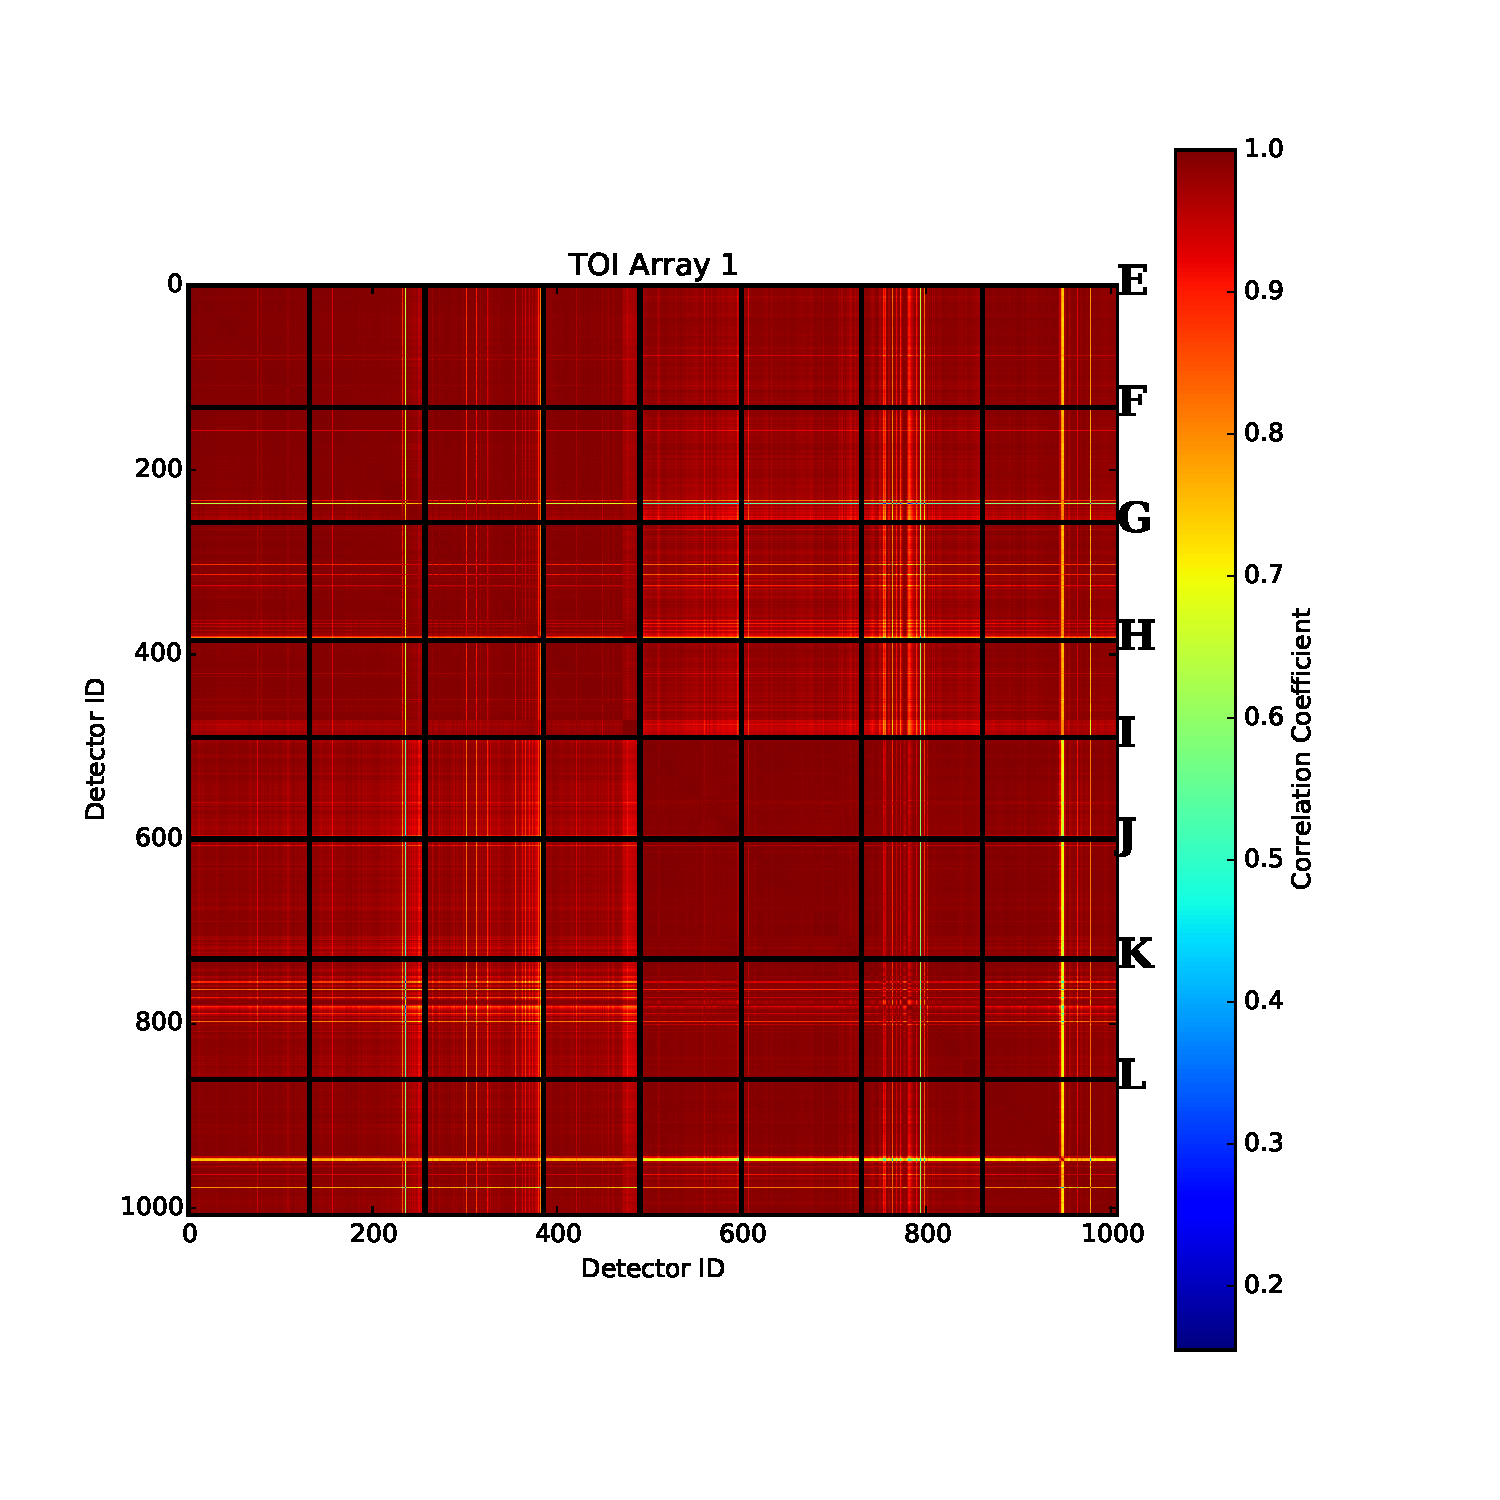
\includegraphics[width=0.3\textwidth]{Figures/NoiseTests/corrmat_TOI_array_1_20170228s151.pdf}
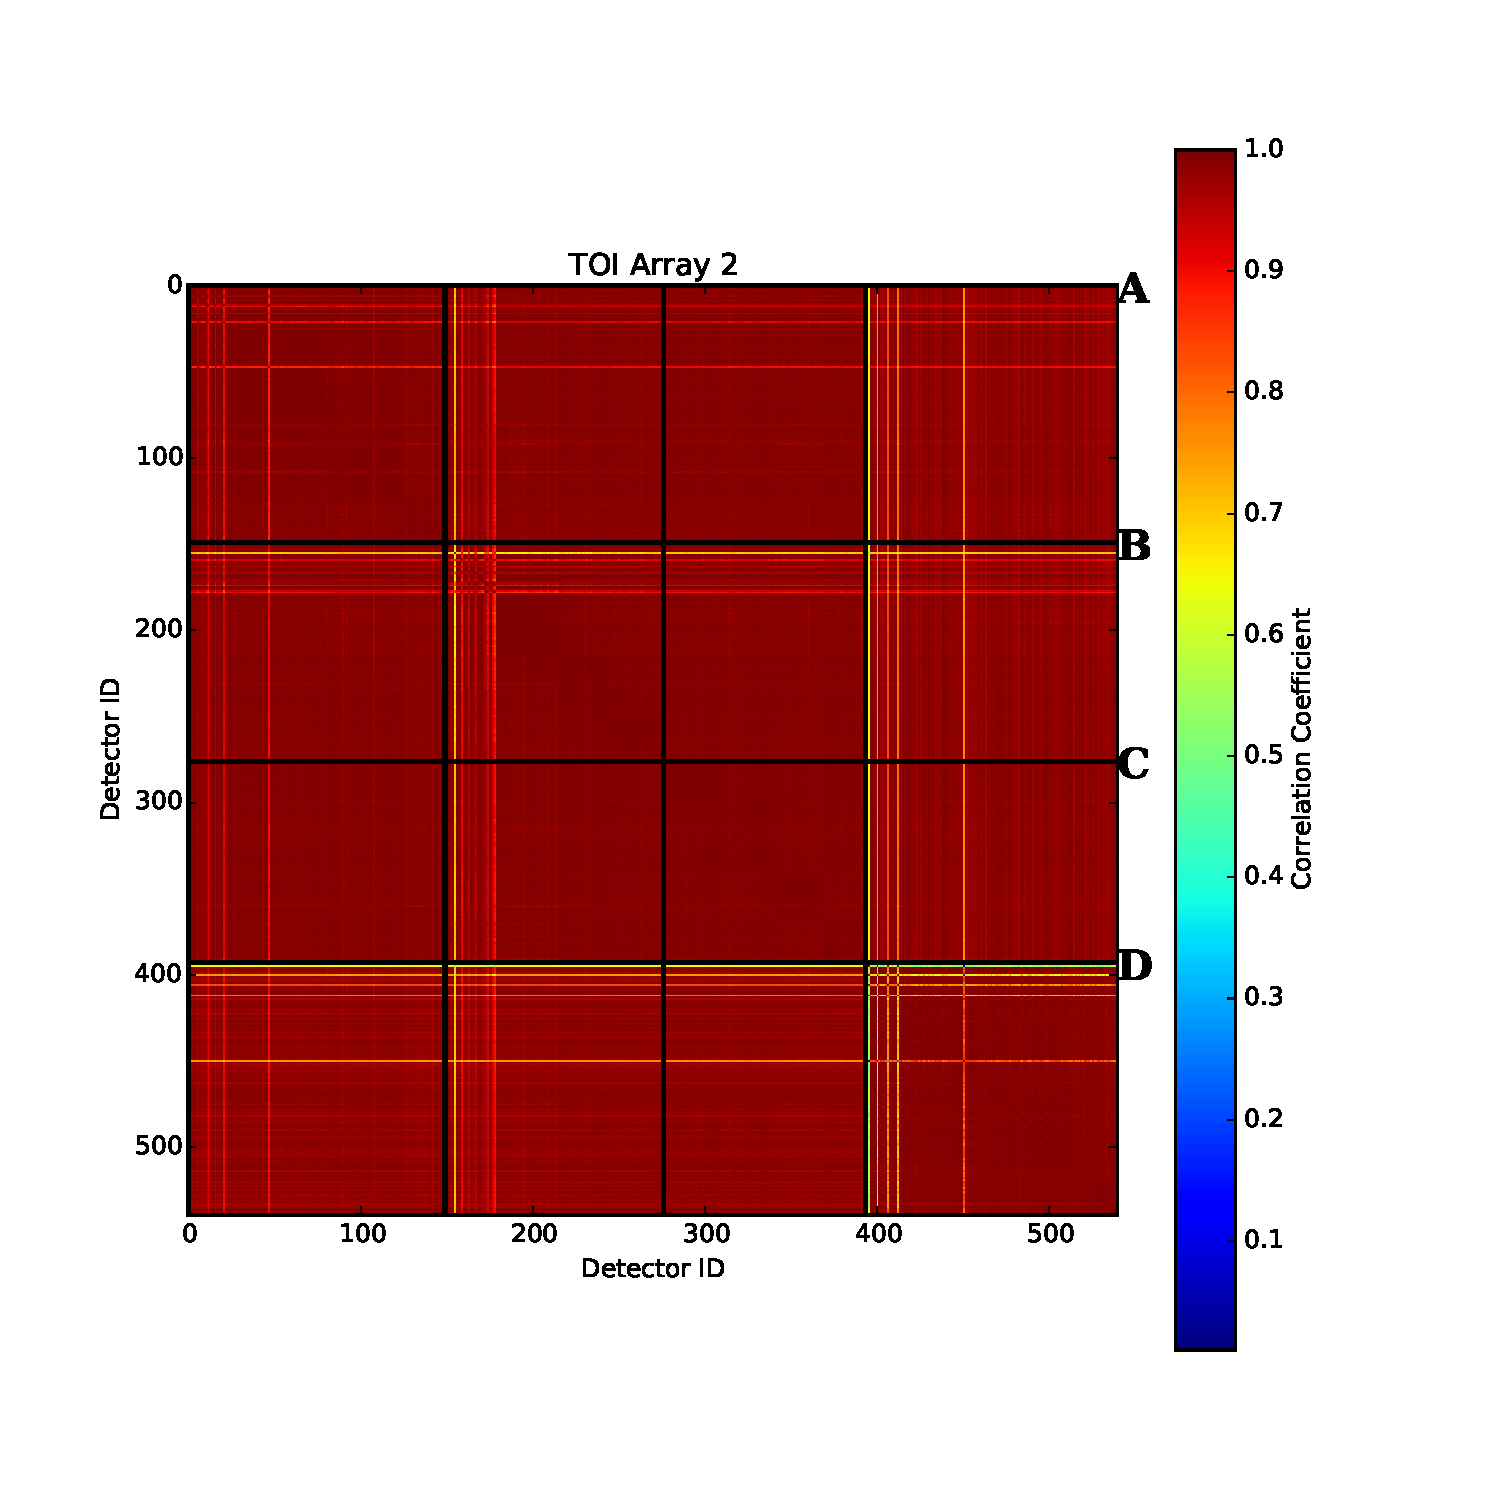
\includegraphics[width=0.3\textwidth]{Figures/NoiseTests/corrmat_TOI_array_2_20170228s151.pdf}
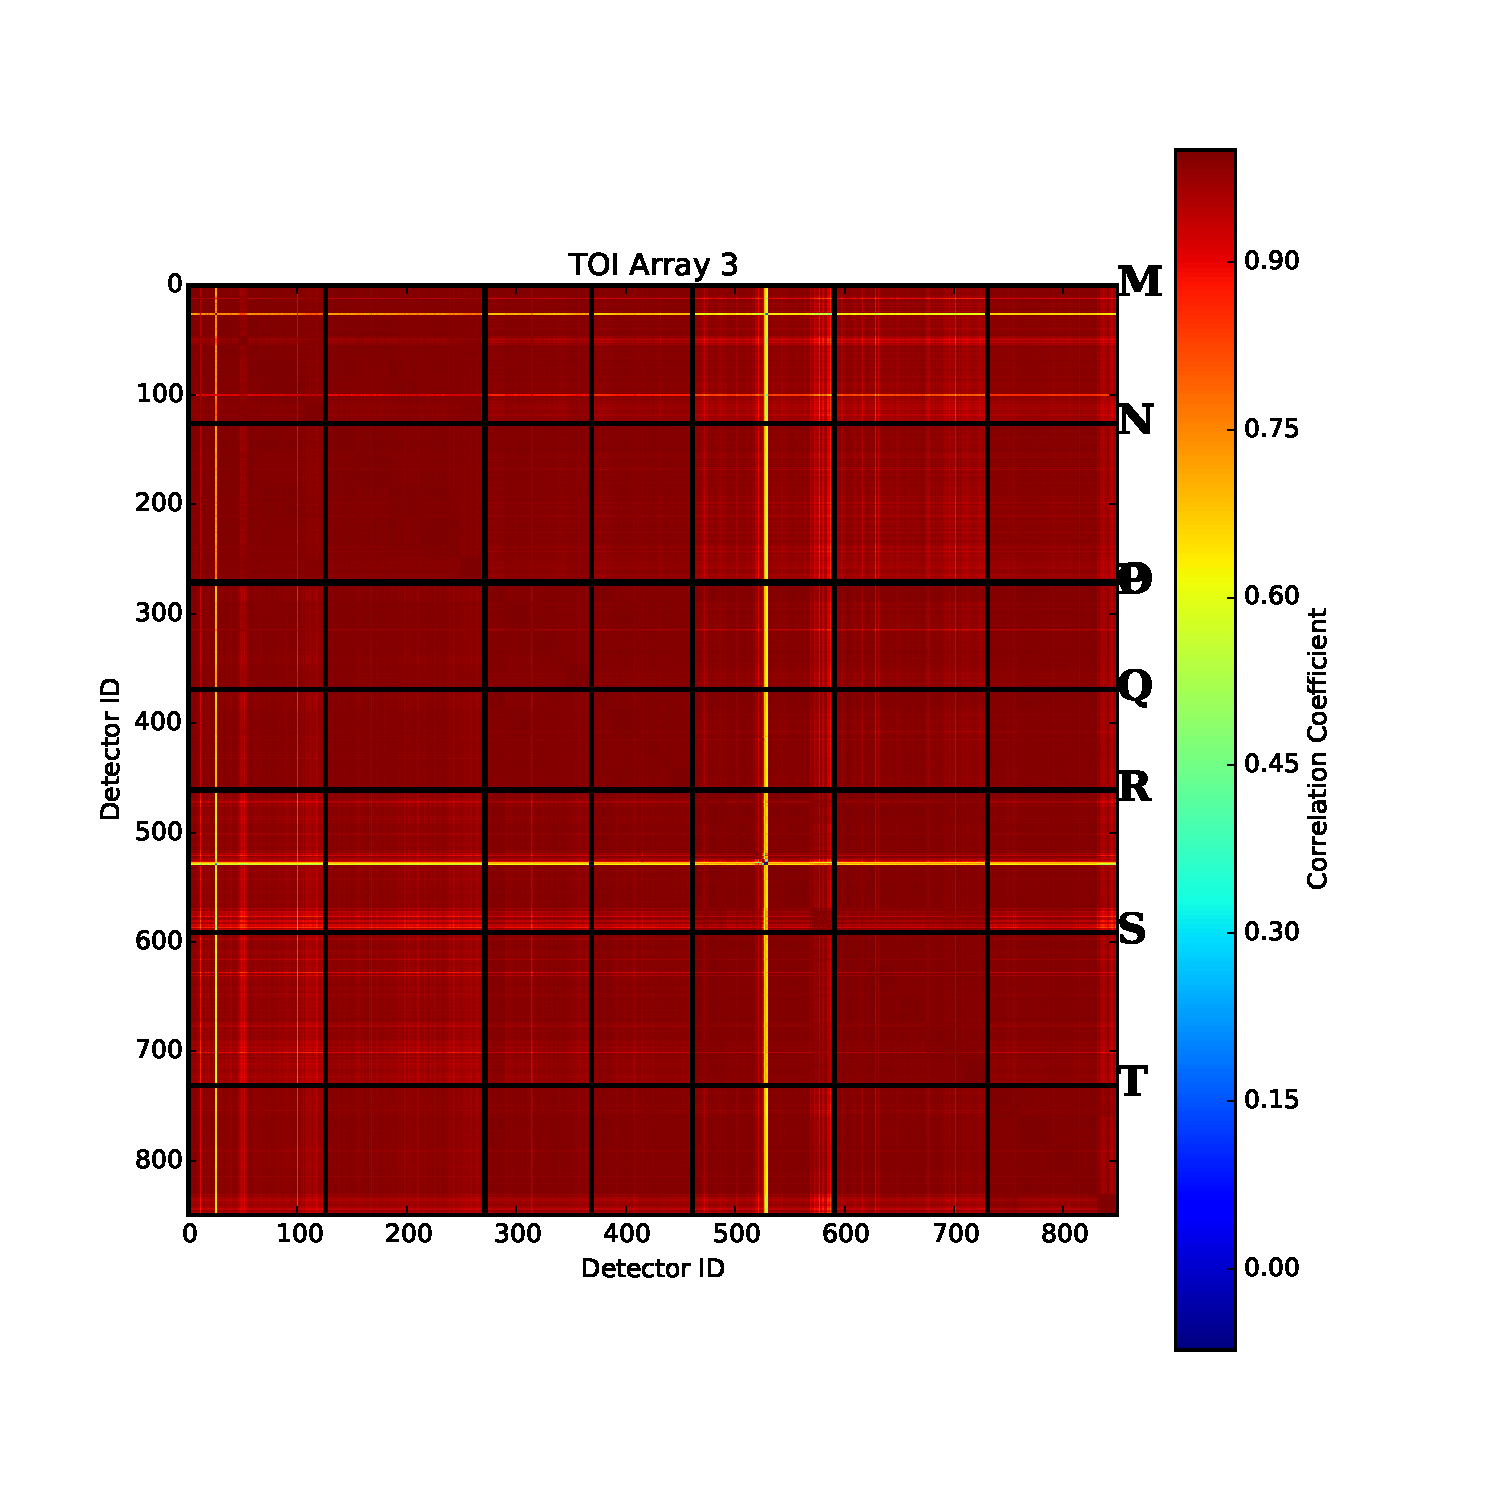
\includegraphics[width=0.3\textwidth]{Figures/NoiseTests/corrmat_TOI_array_3_20170228s151.pdf}
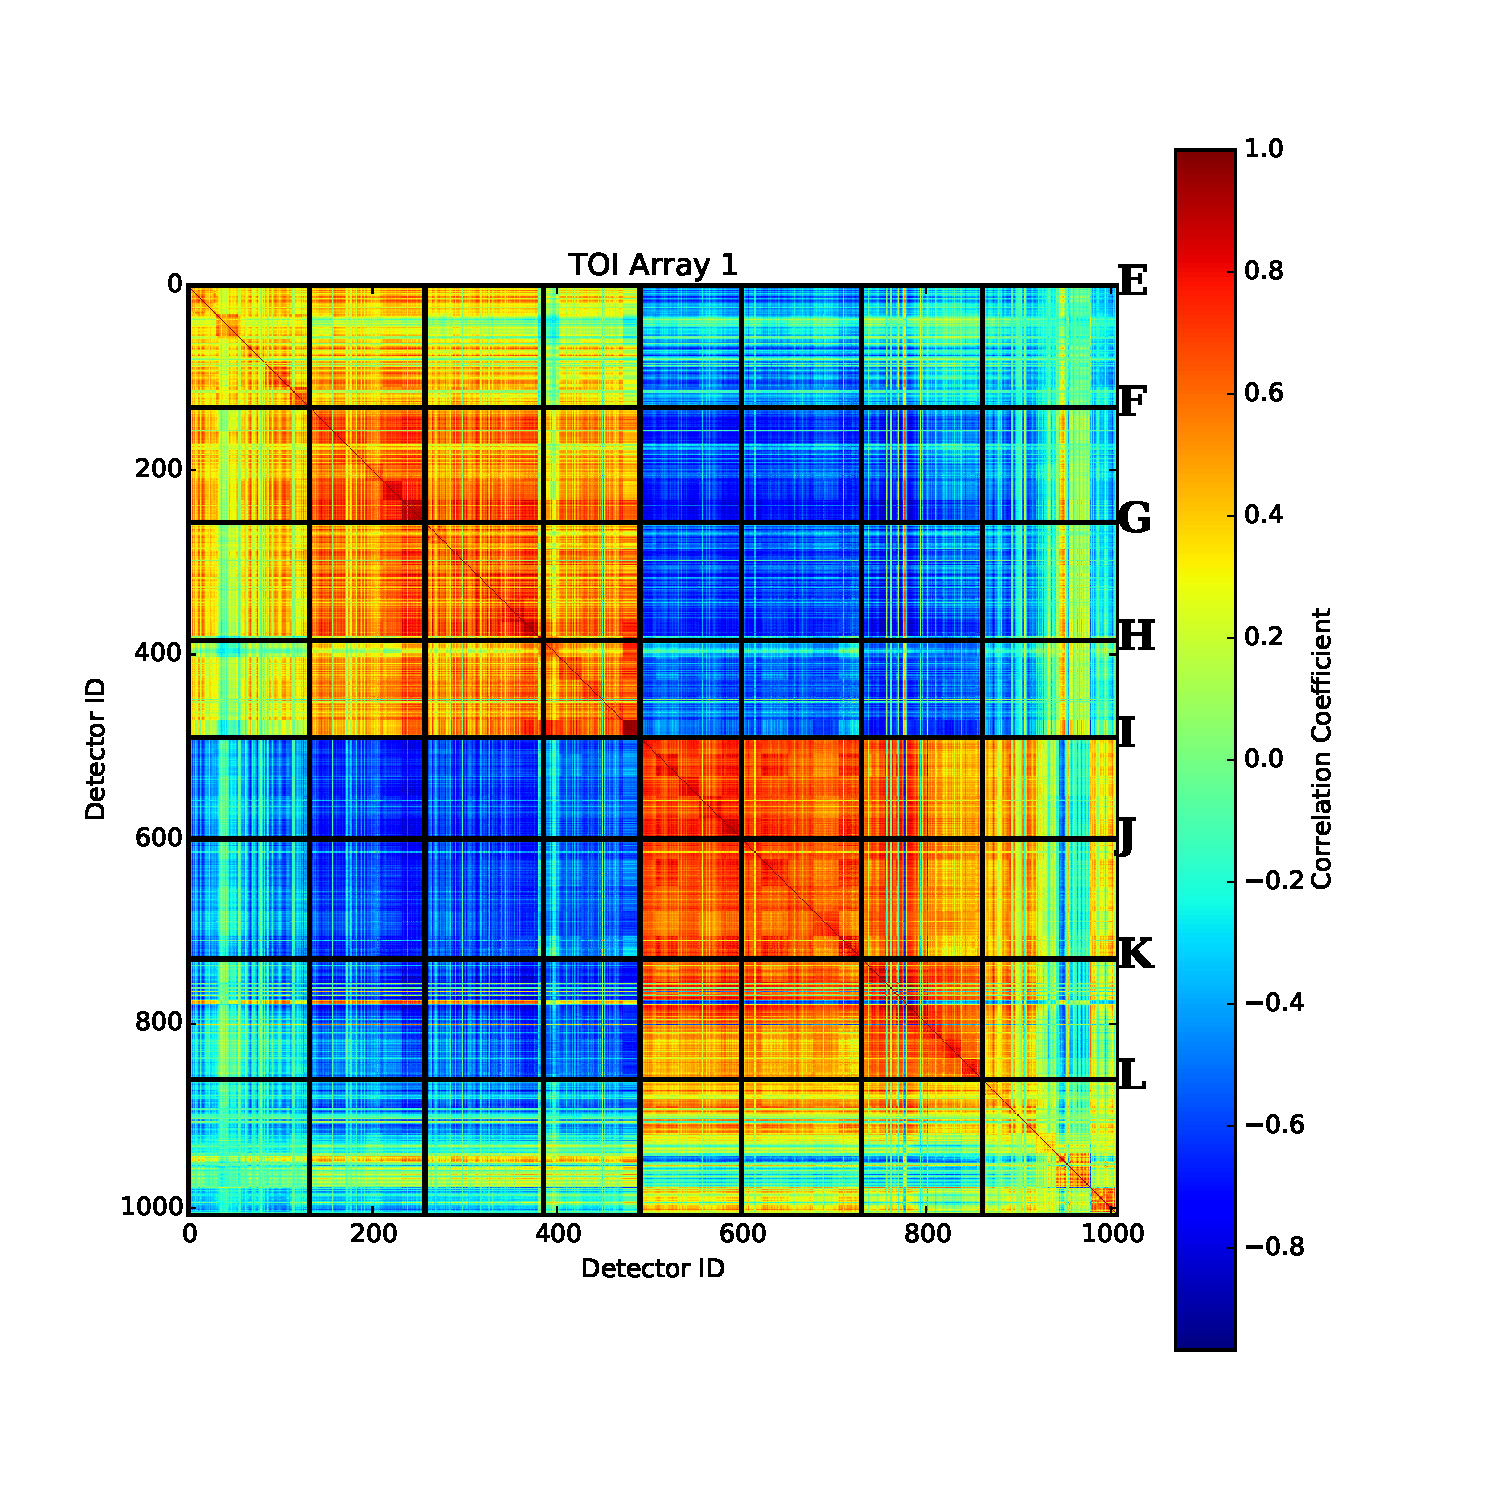
\includegraphics[width=0.3\textwidth]{Figures/NoiseTests/corrmat_TOI_CM_array_1_20170228s151.pdf}
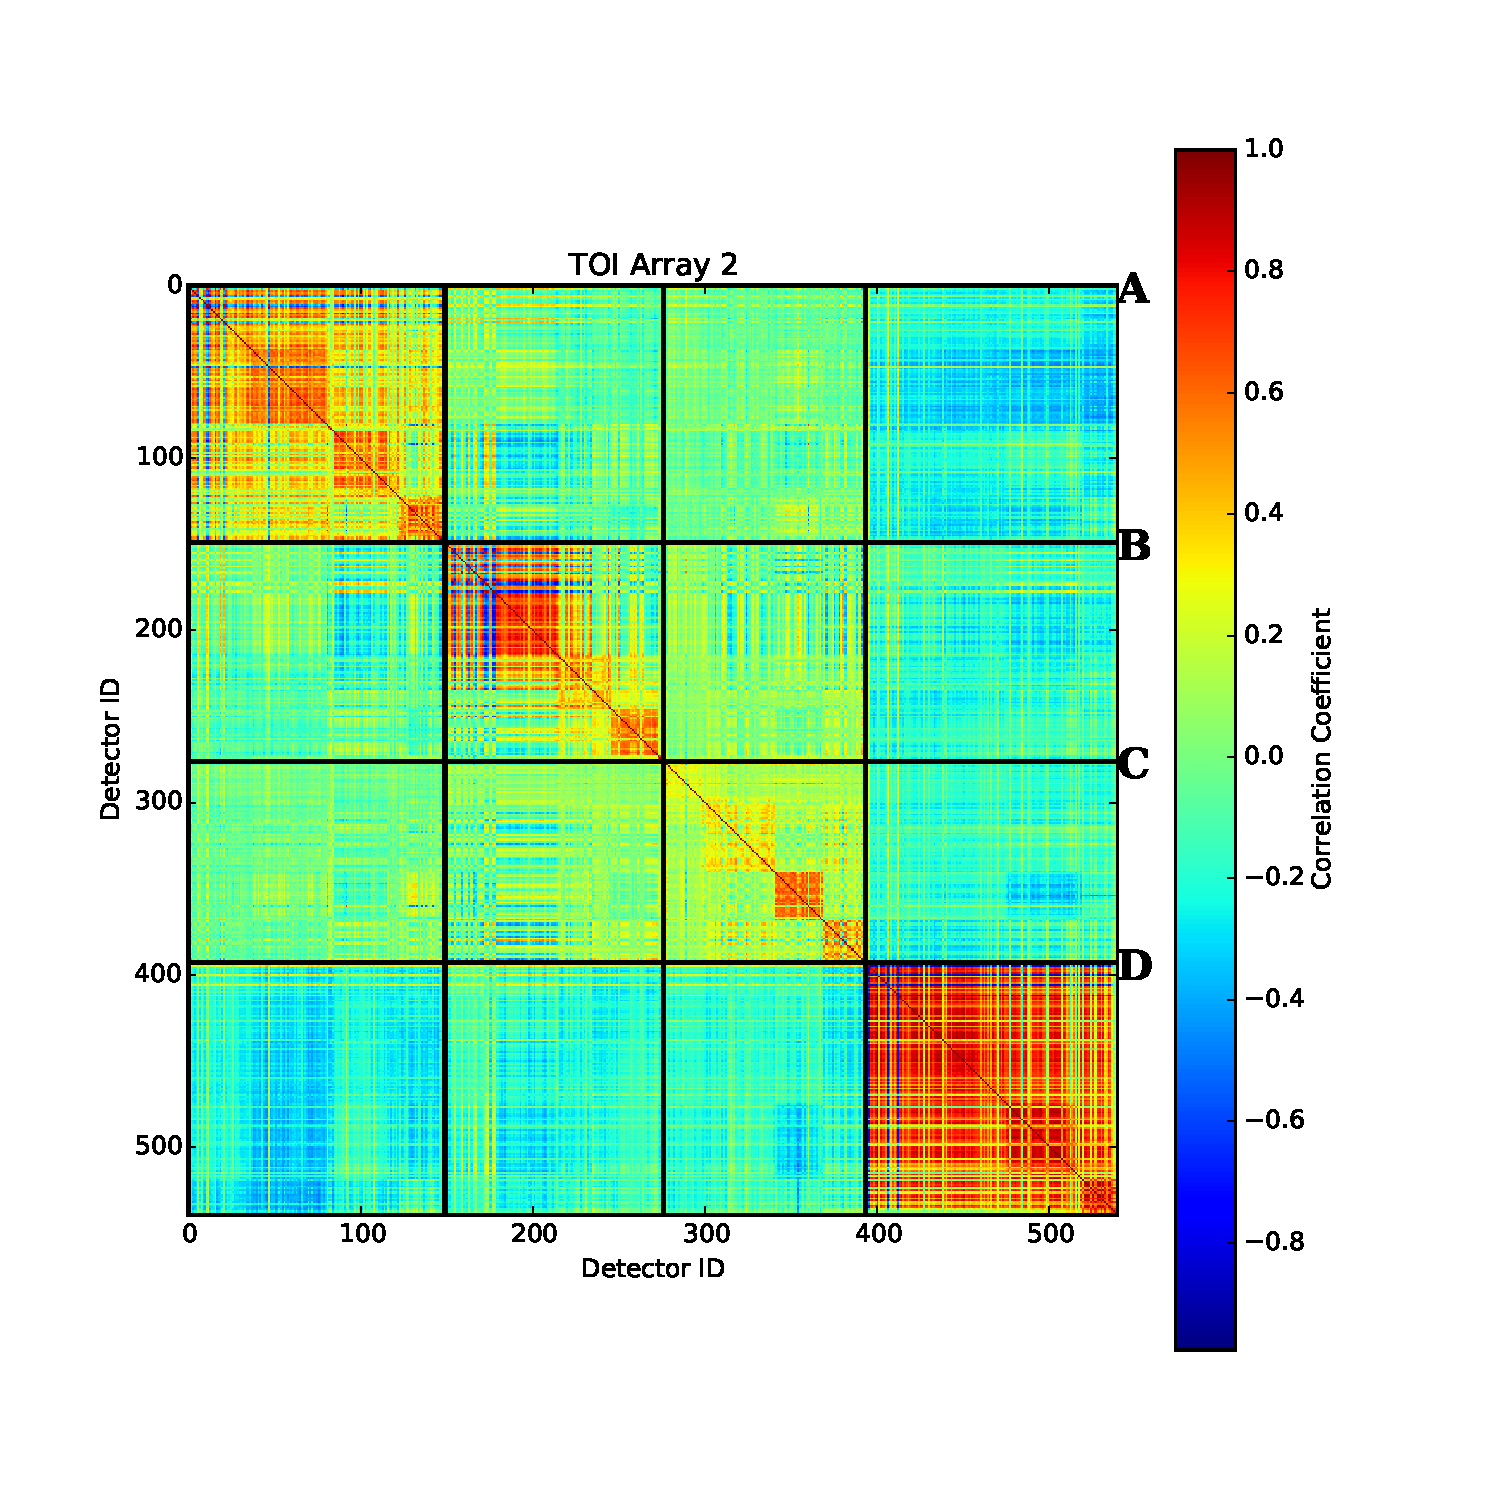
\includegraphics[width=0.3\textwidth]{Figures/NoiseTests/corrmat_TOI_CM_array_2_20170228s151.pdf}
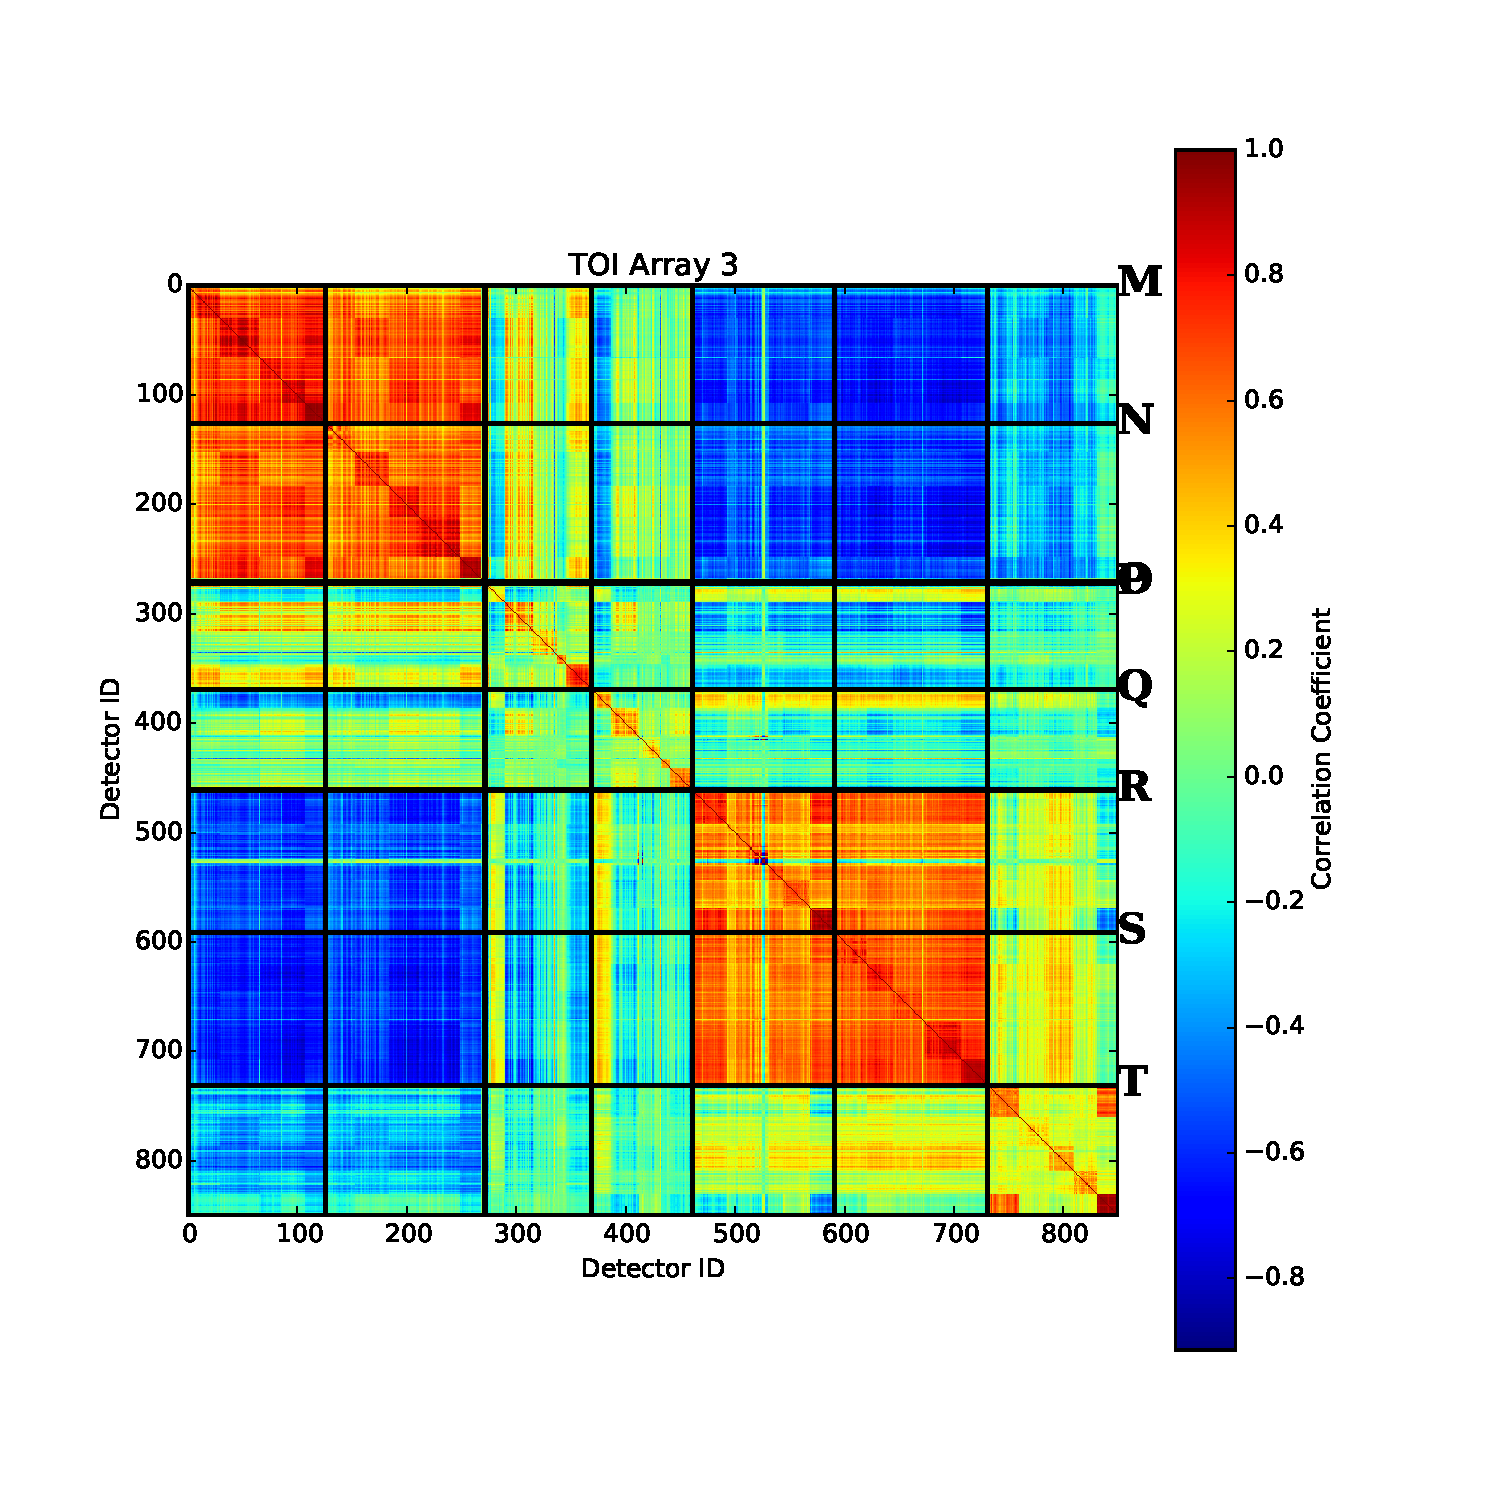
\includegraphics[width=0.3\textwidth]{Figures/NoiseTests/corrmat_TOI_CM_array_3_20170228s151.pdf}
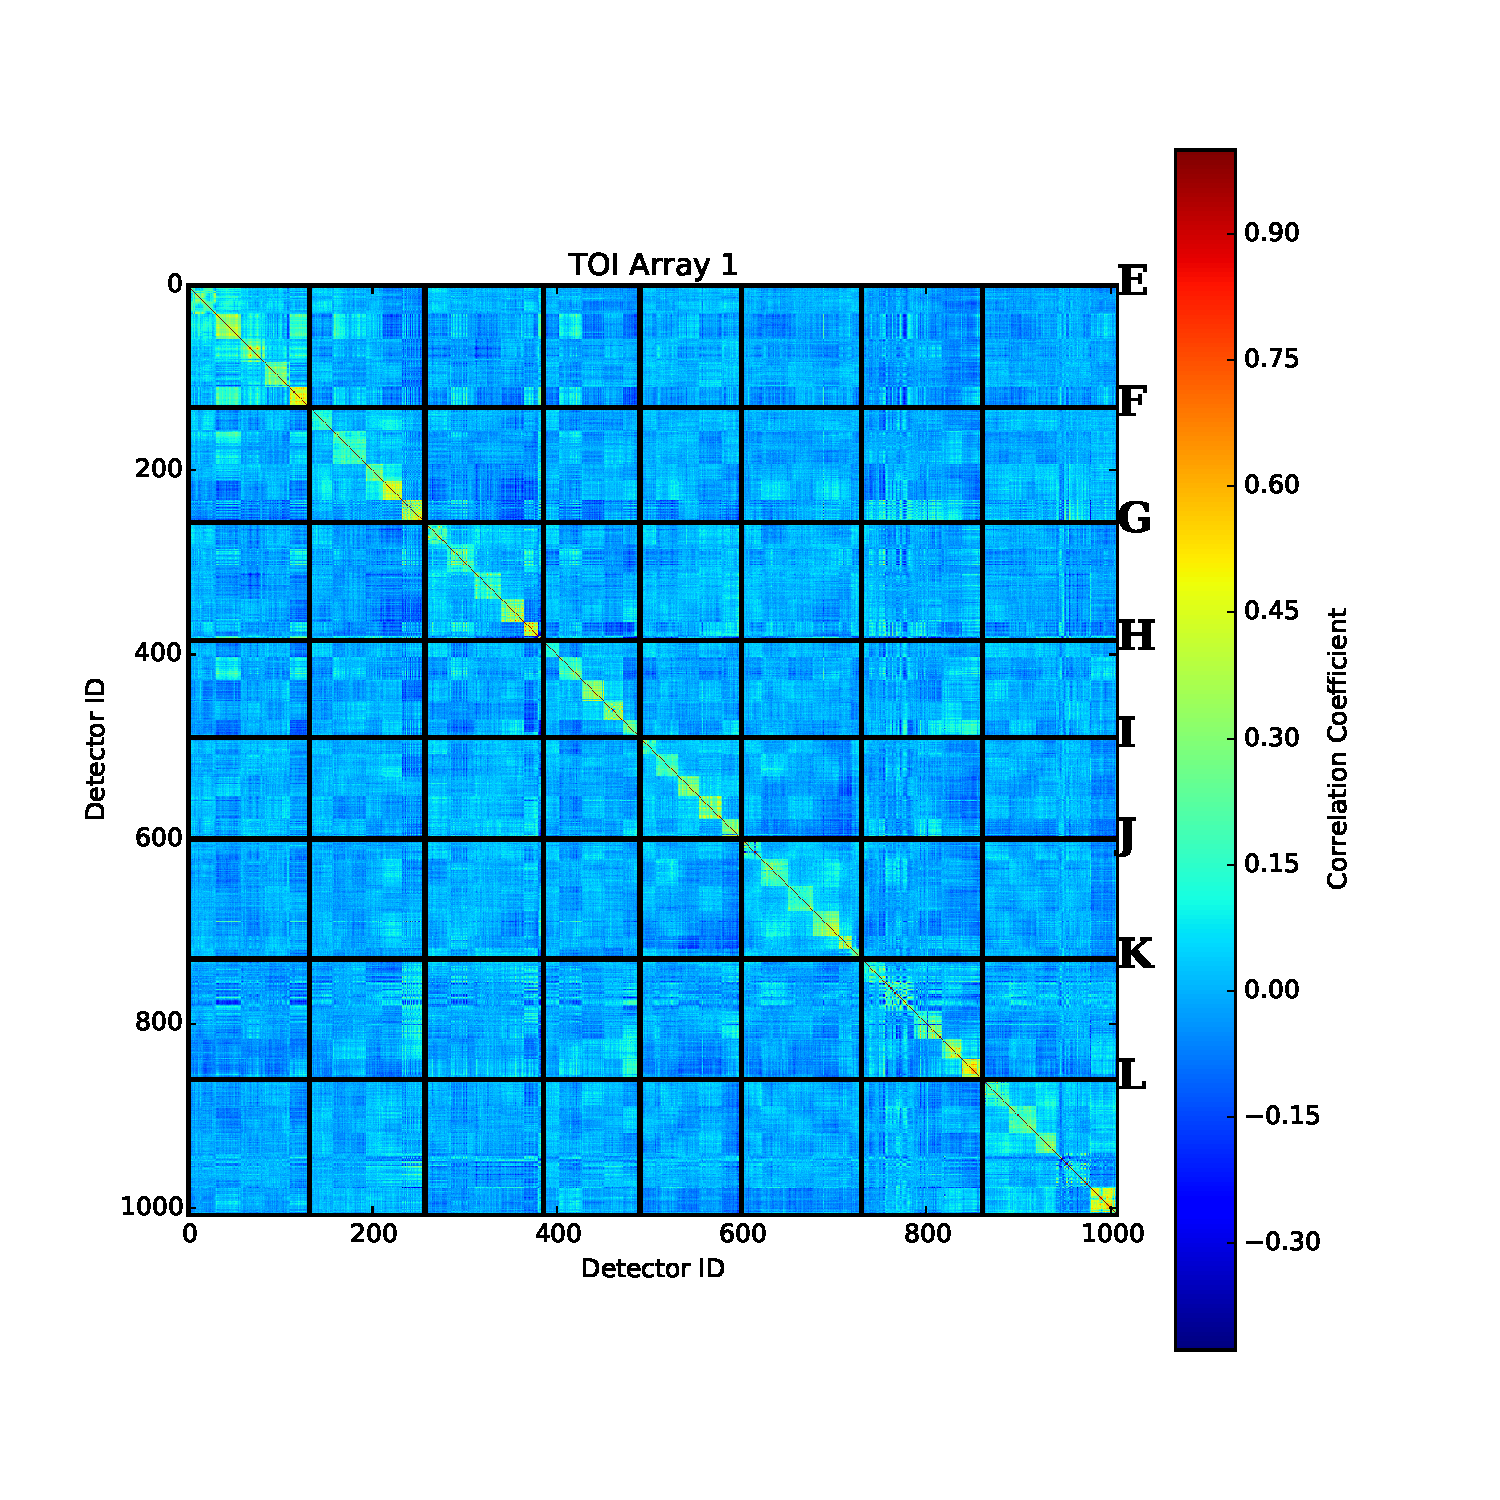
\includegraphics[width=0.3\textwidth]{Figures/NoiseTests/corrmat_TOI_PCA_array_1_20170228s151.pdf}
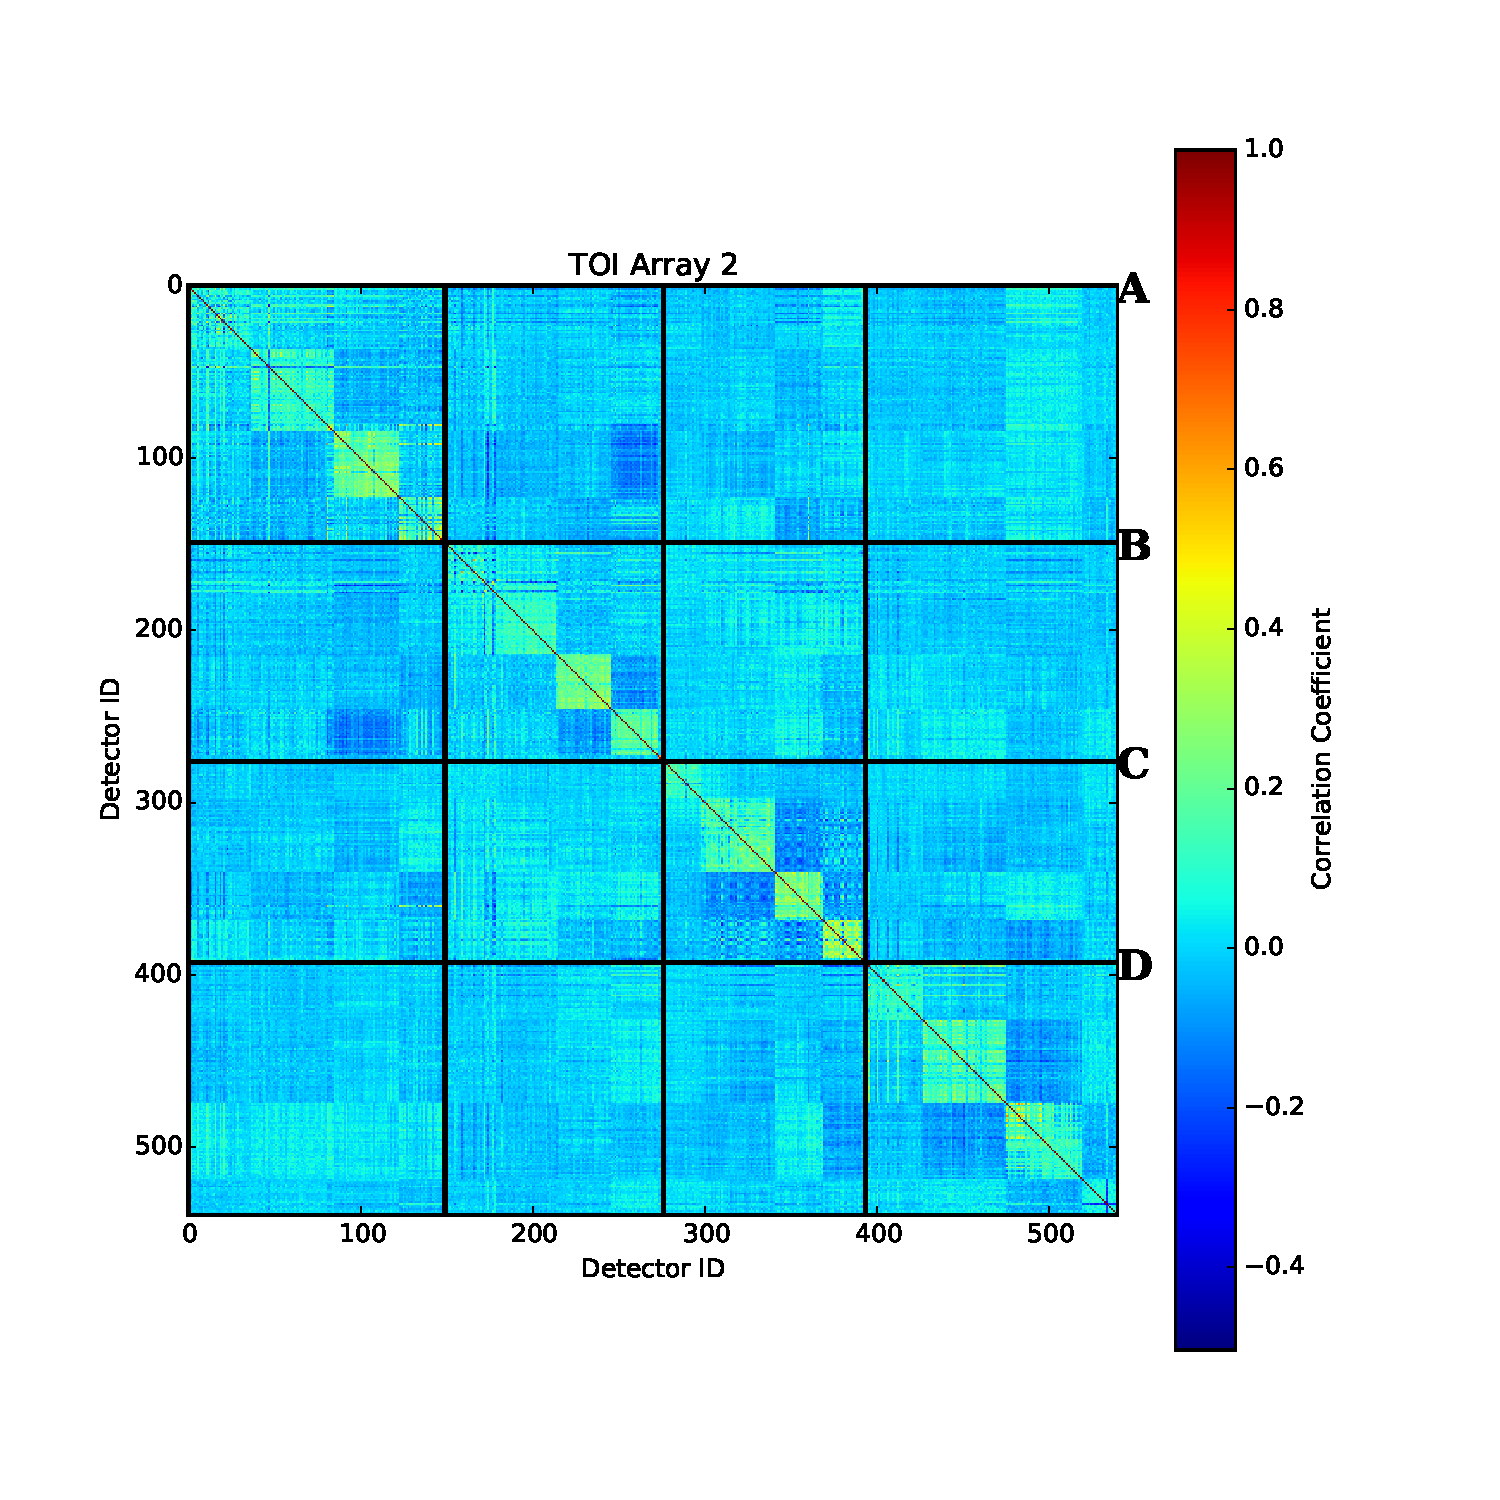
\includegraphics[width=0.3\textwidth]{Figures/NoiseTests/corrmat_TOI_PCA_array_2_20170228s151.pdf}
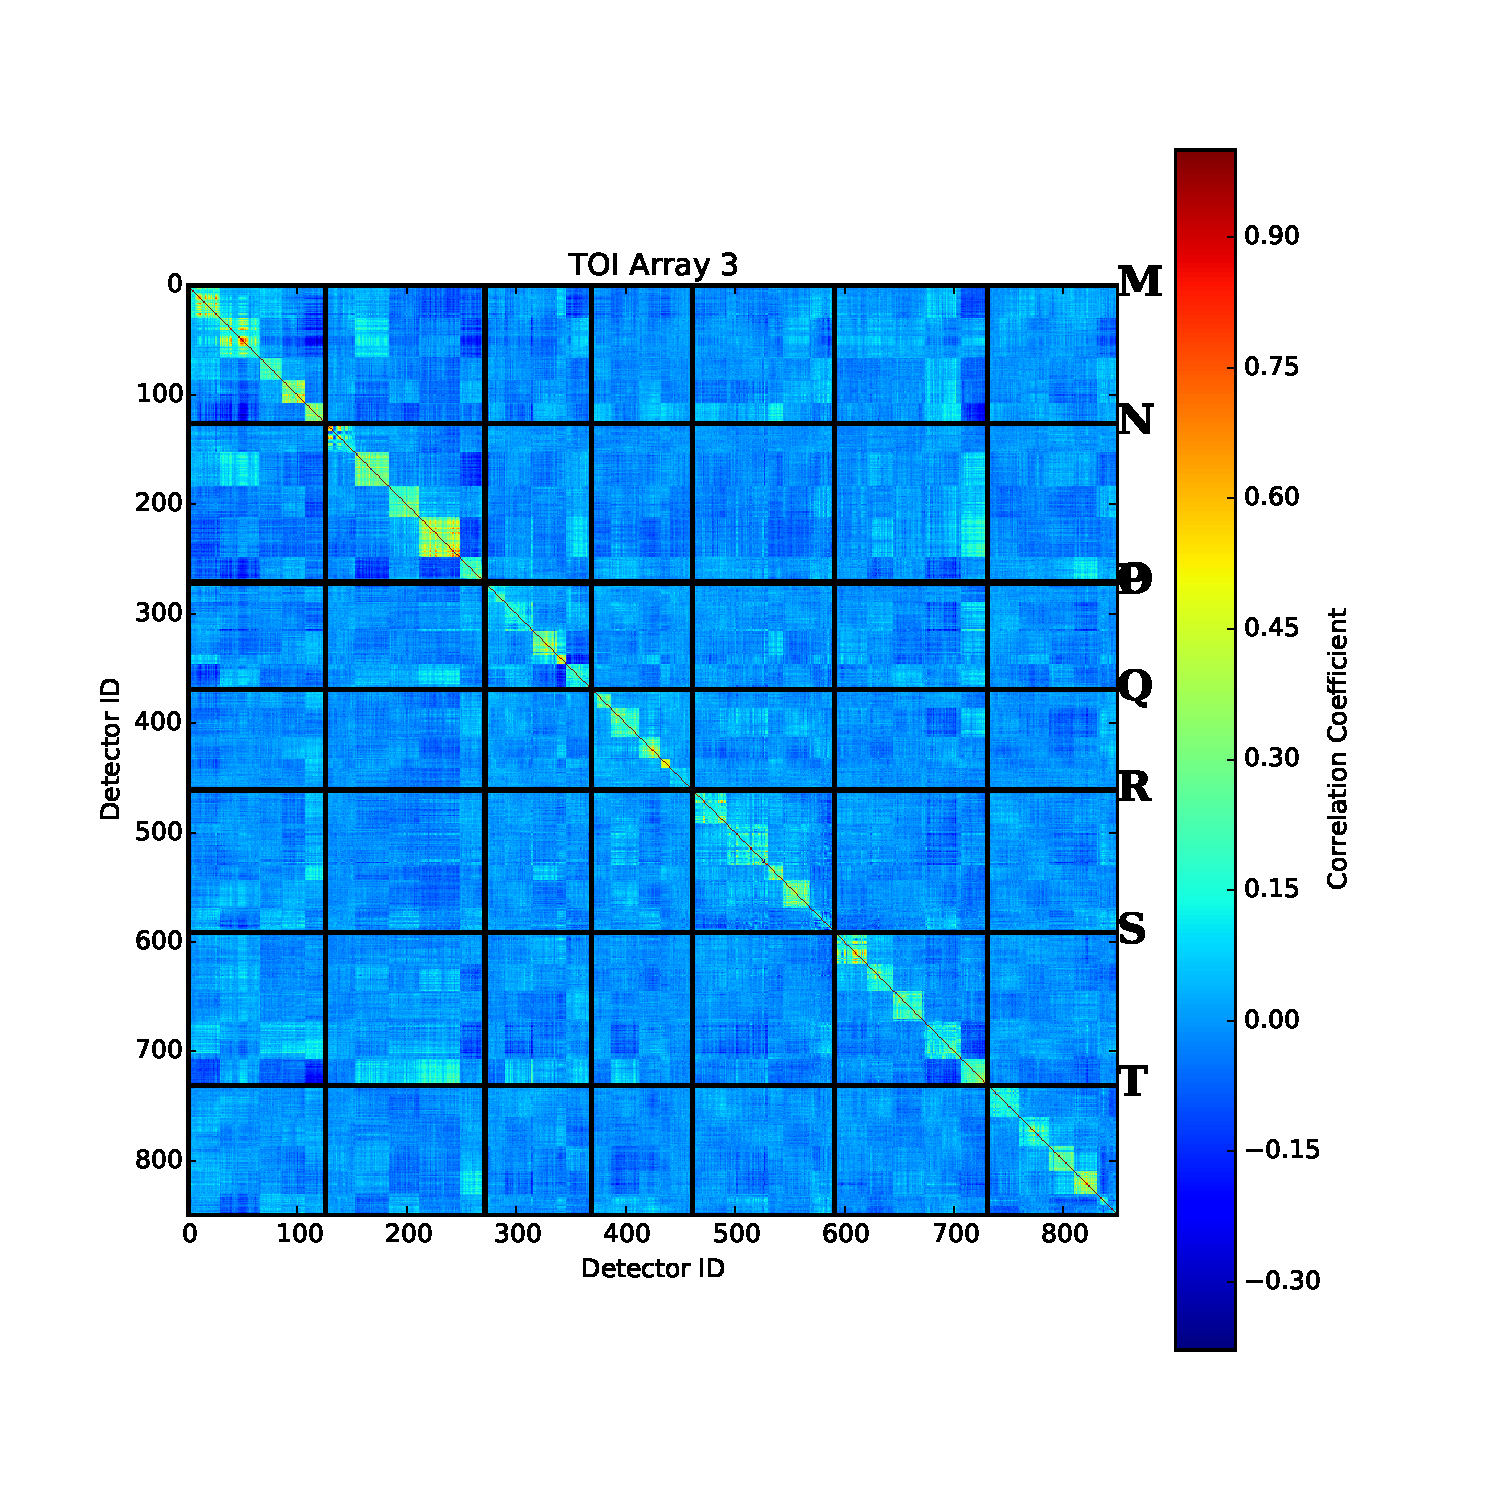
\includegraphics[width=0.3\textwidth]{Figures/NoiseTests/corrmat_TOI_PCA_array_3_20170228s151.pdf}
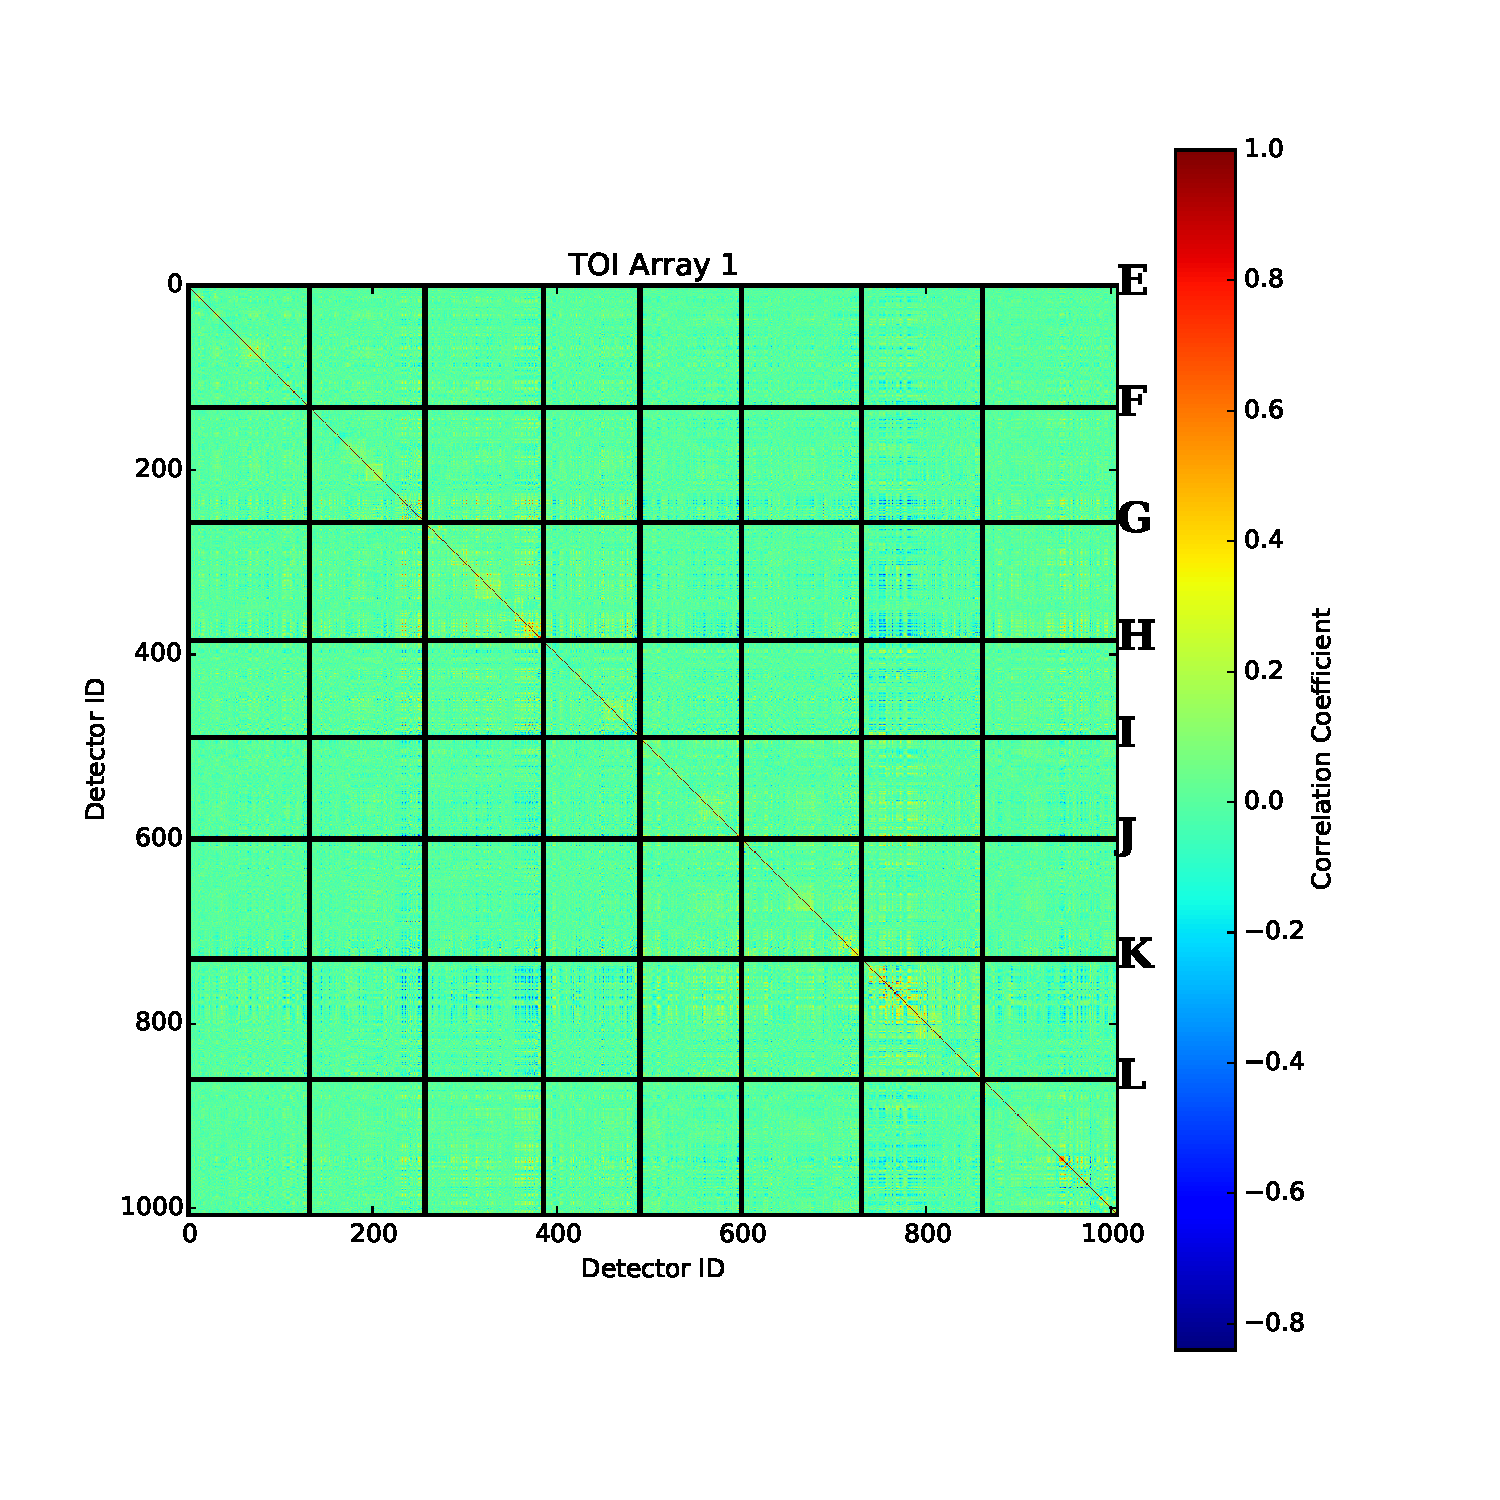
\includegraphics[width=0.3\textwidth]{Figures/NoiseTests/corrmat_TOI_BCP_array_1_20170228s151.pdf}
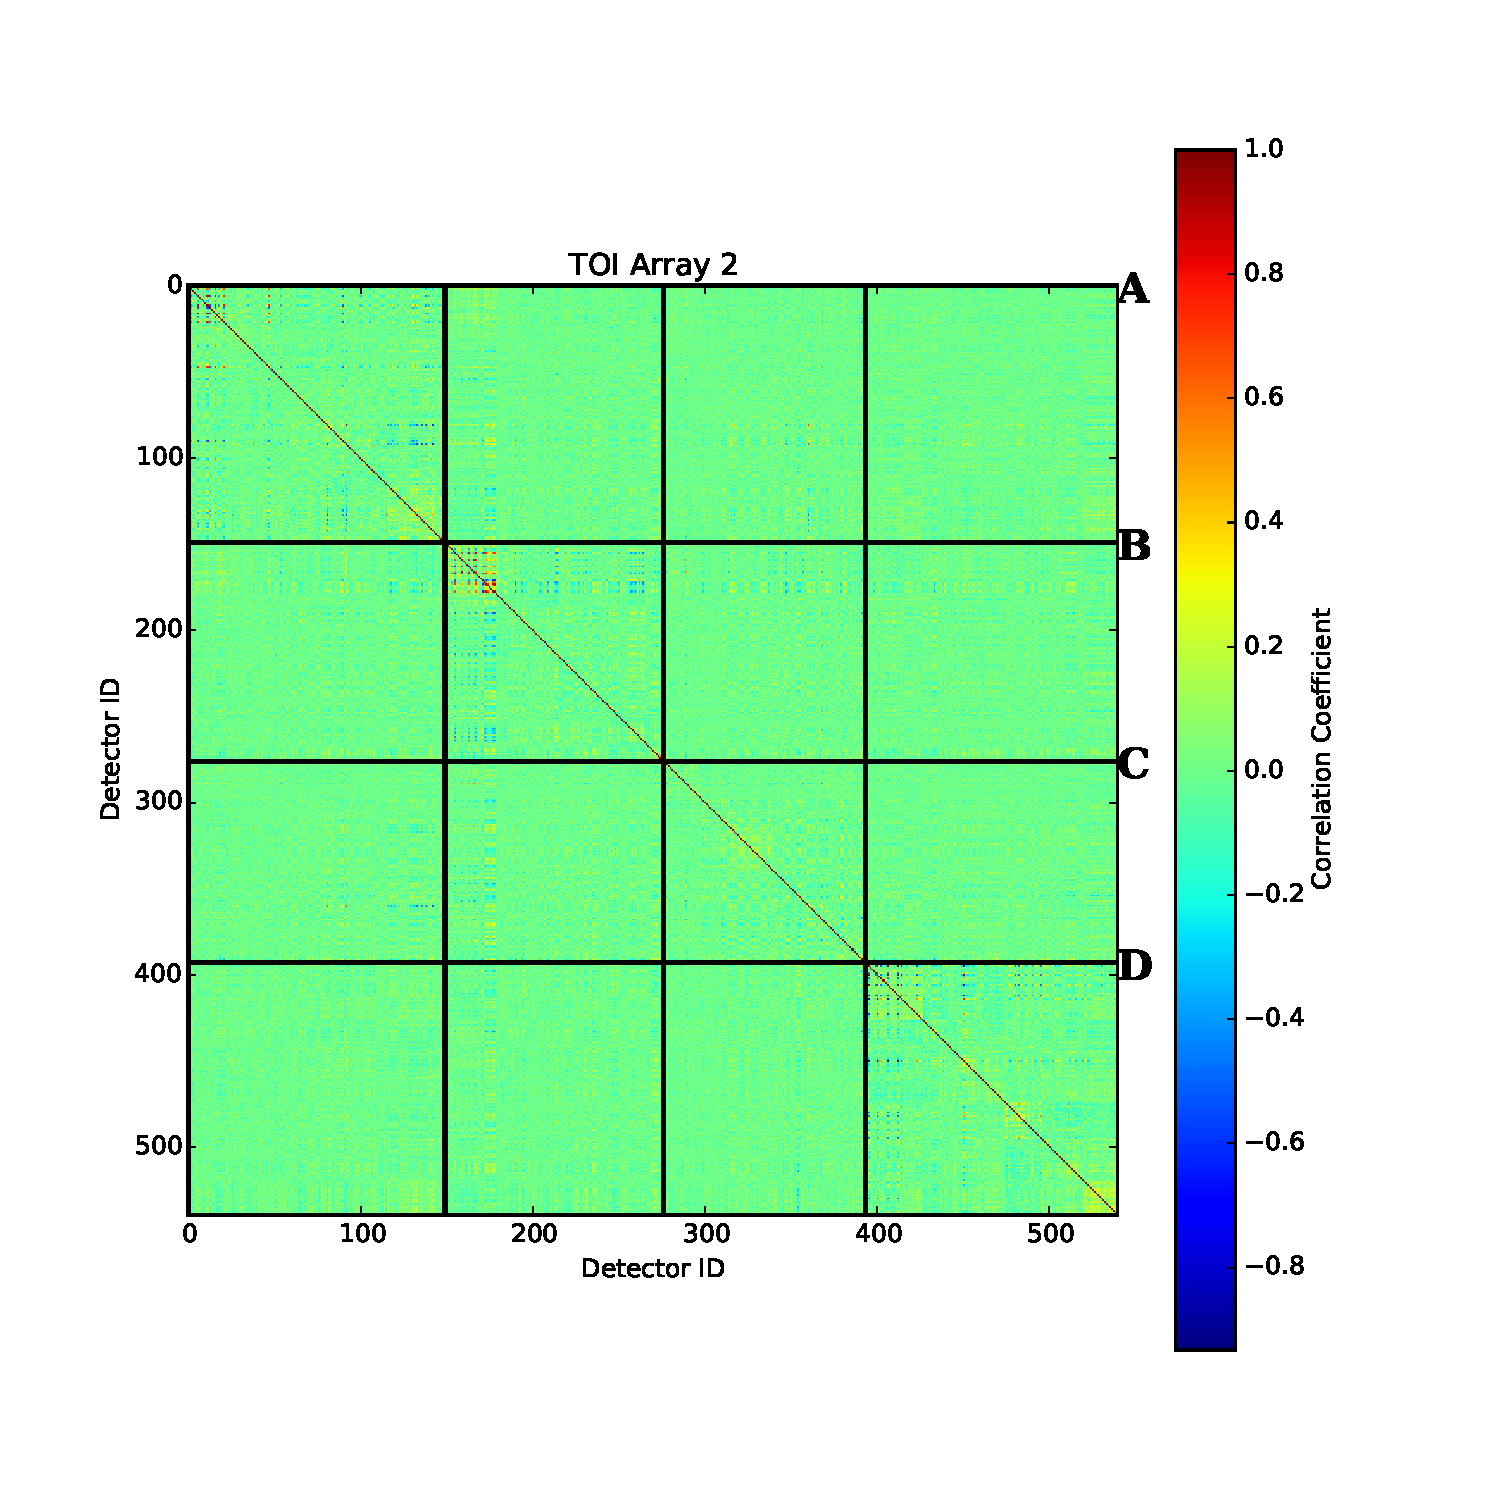
\includegraphics[width=0.3\textwidth]{Figures/NoiseTests/corrmat_TOI_BCP_array_2_20170228s151.pdf}
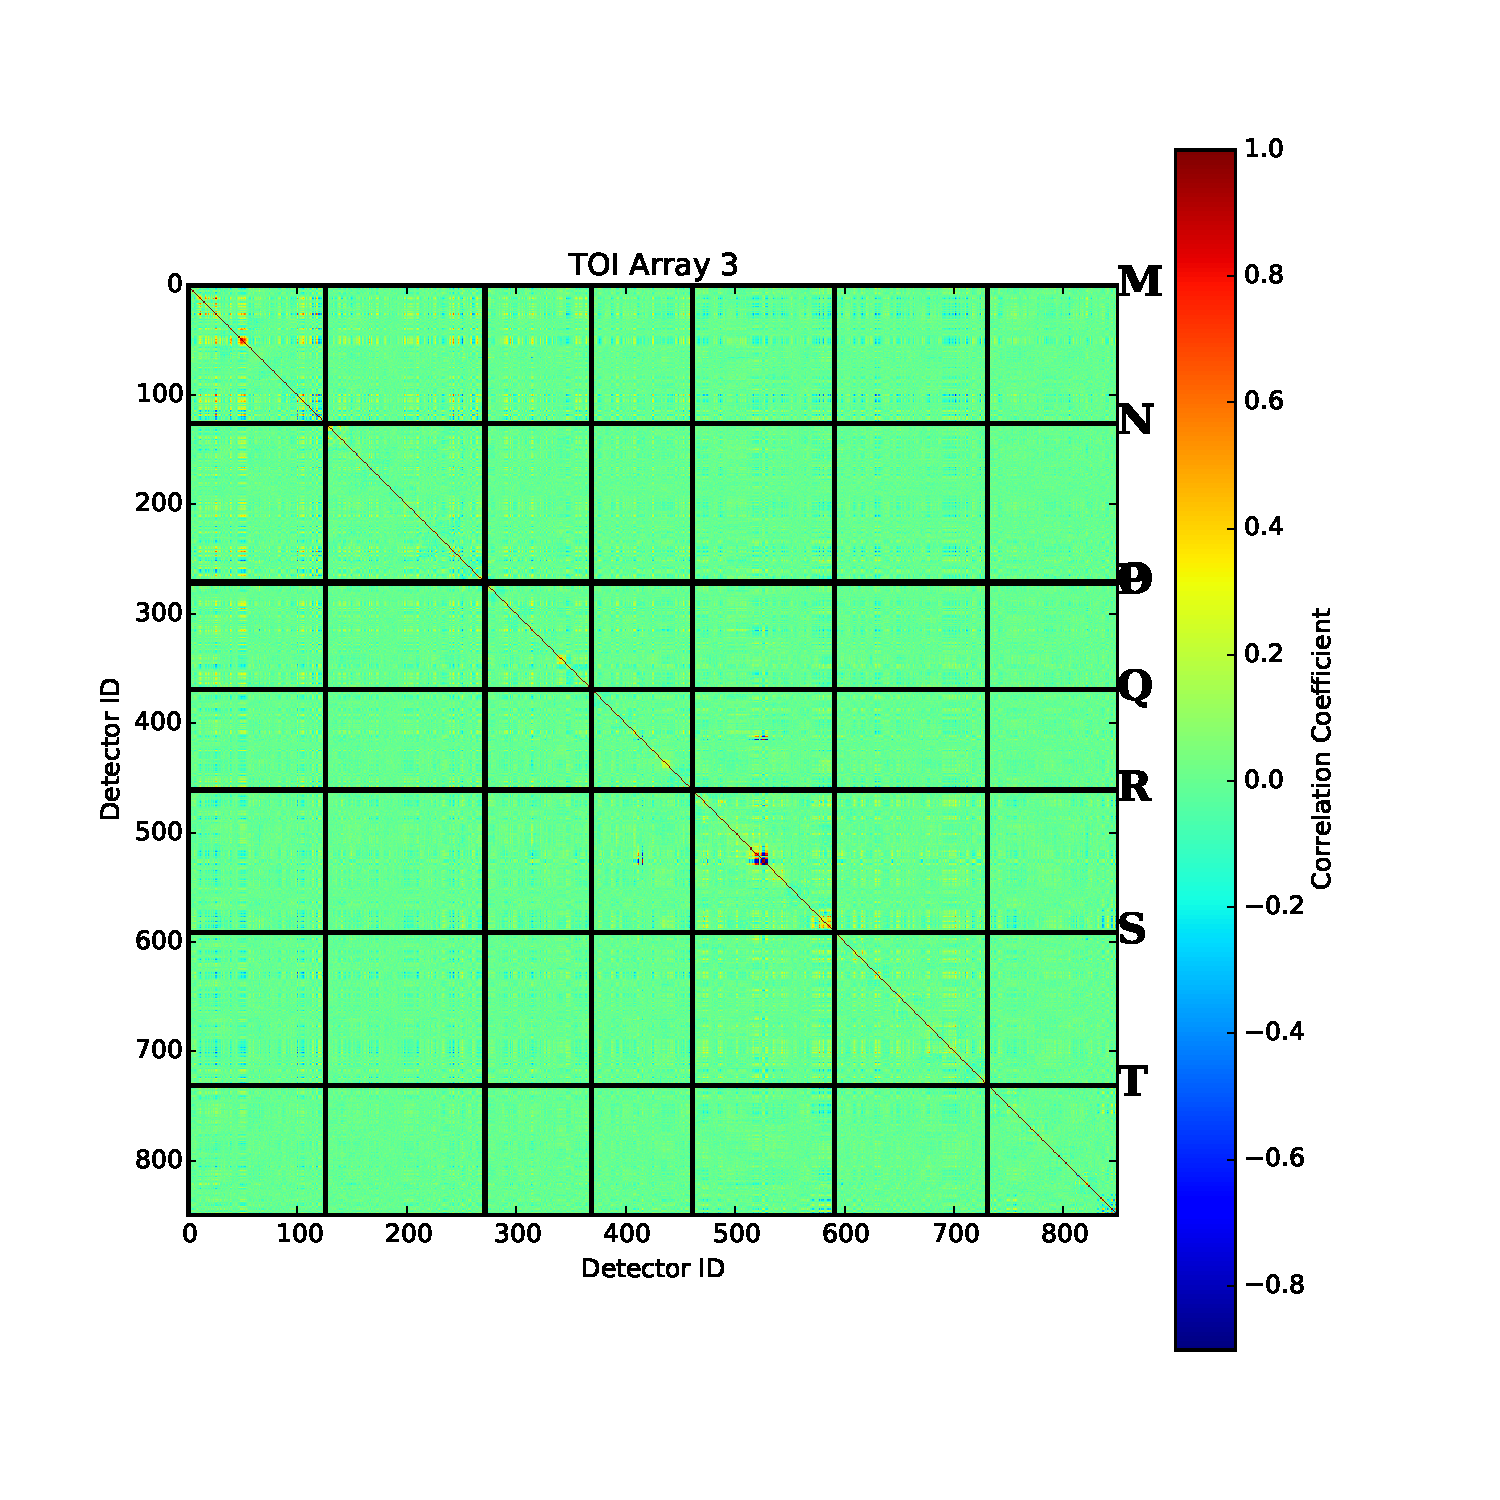
\includegraphics[width=0.3\textwidth]{Figures/NoiseTests/corrmat_TOI_BCP_array_3_20170228s151.pdf}
\end{center}
\caption[KID-to-KID correlation matrices]{From left to right correlation matrices for the three NIKA2 arrays (A1, A2, and A3) for scan 20170228s150. From top to bottom we present the correlation of the raw data, after CM, PCA and BCP decorrelation methods. \label{corrmatrix}}
\end{figure}



\subsection{RMS noise and power spectra}

\begin{figure}[ht] % Inline image example
\begin{center}
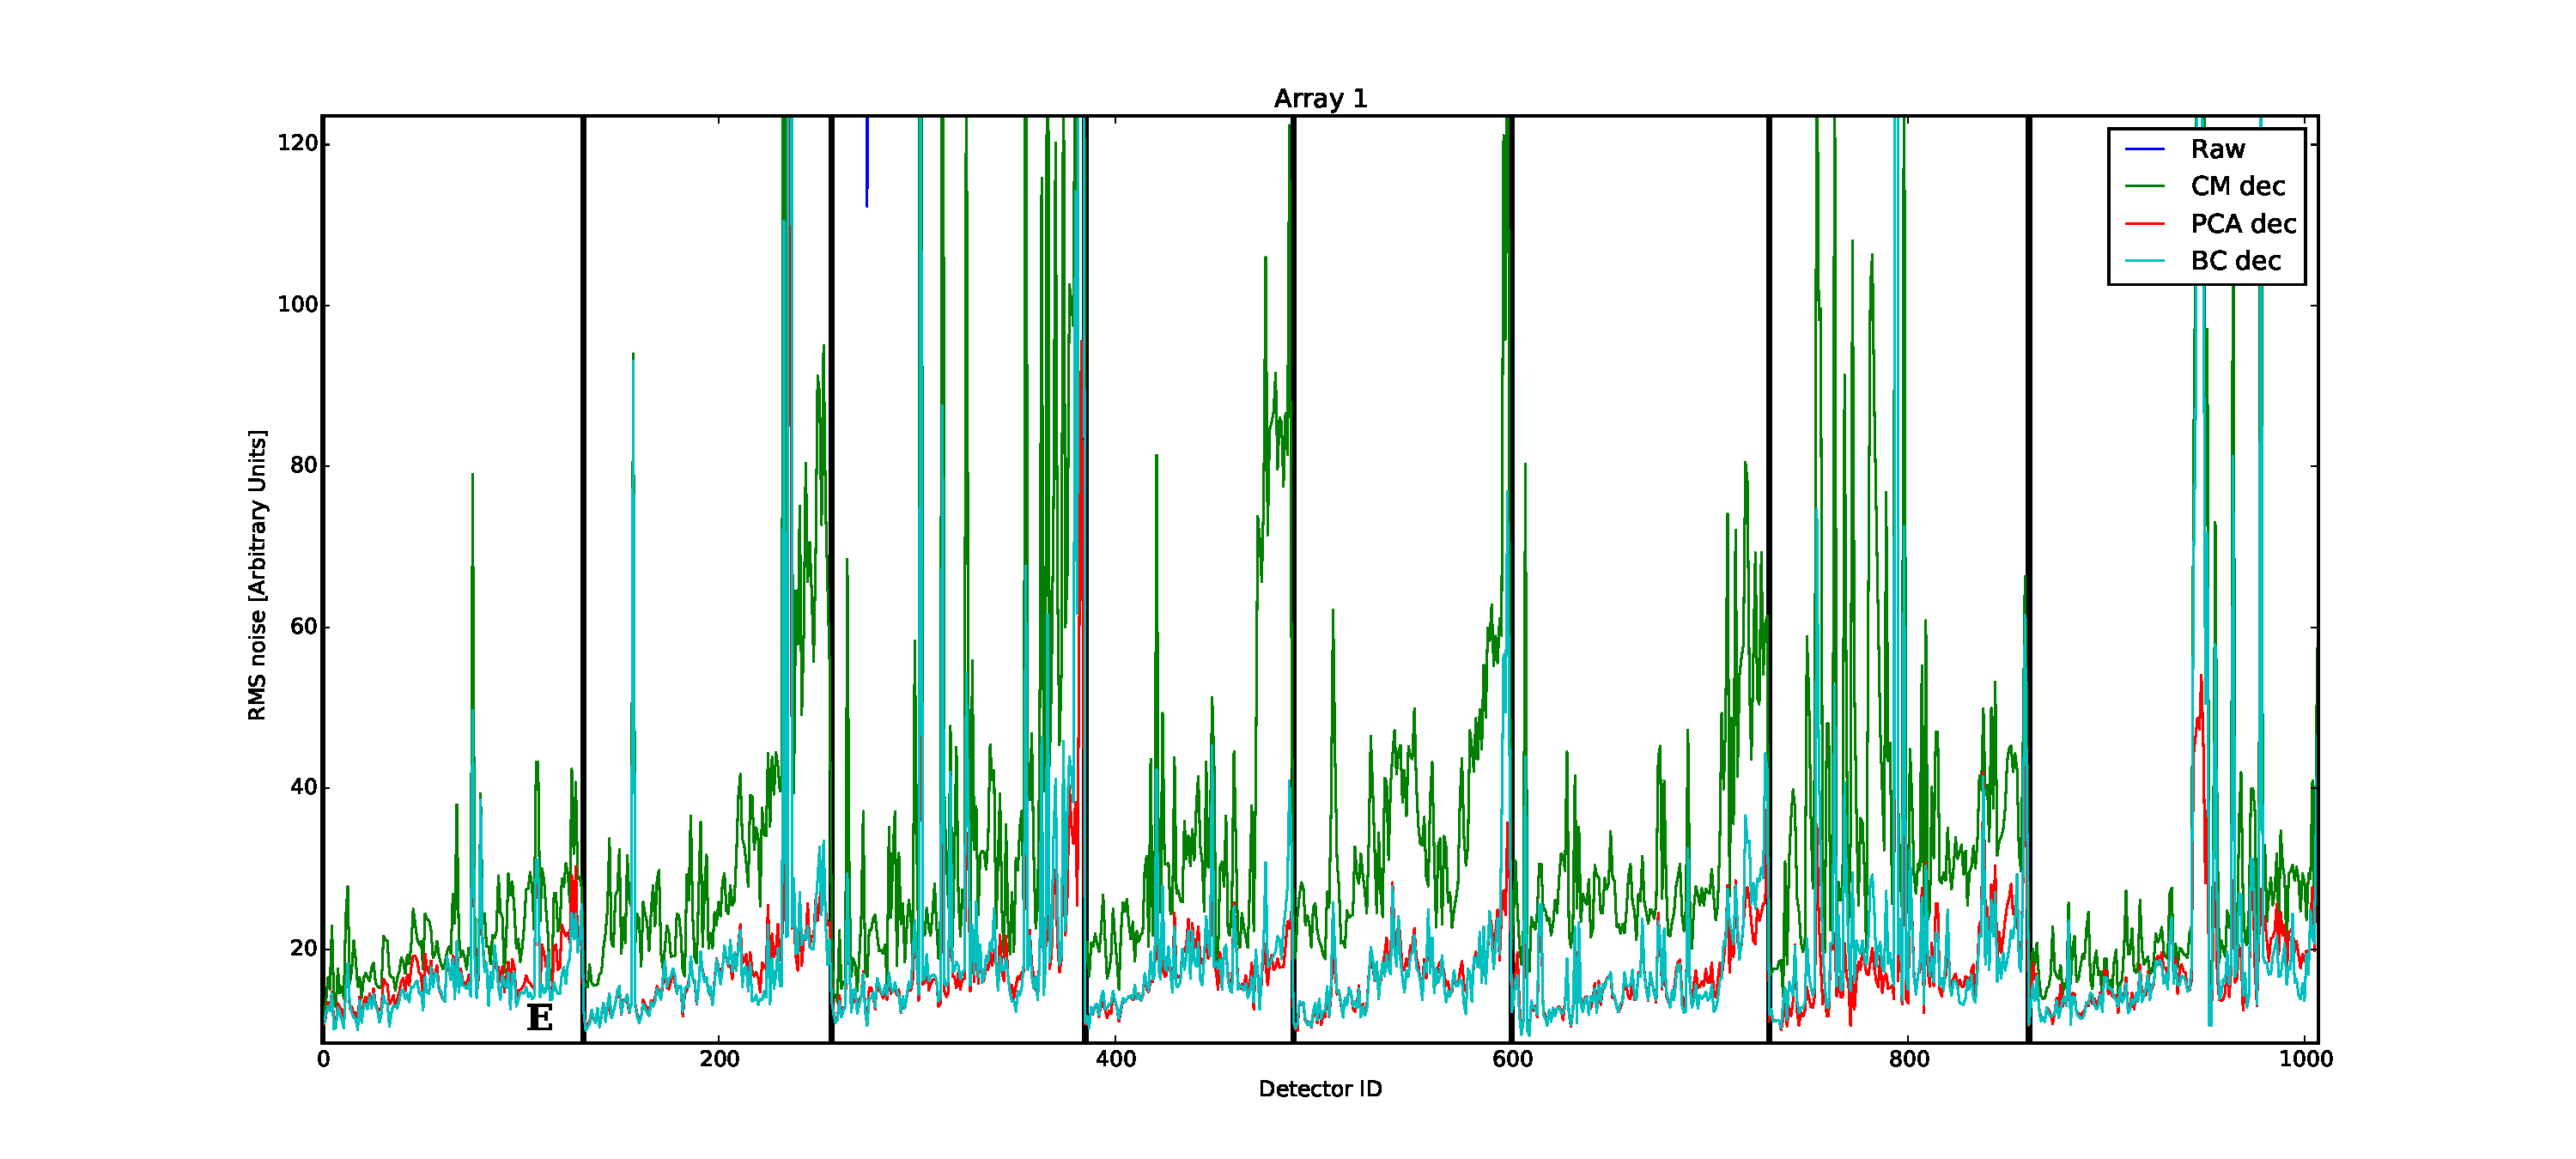
\includegraphics[width=0.3\textwidth]{Figures/NoiseTests/rms_TOI_array_1_20170228s151.pdf}
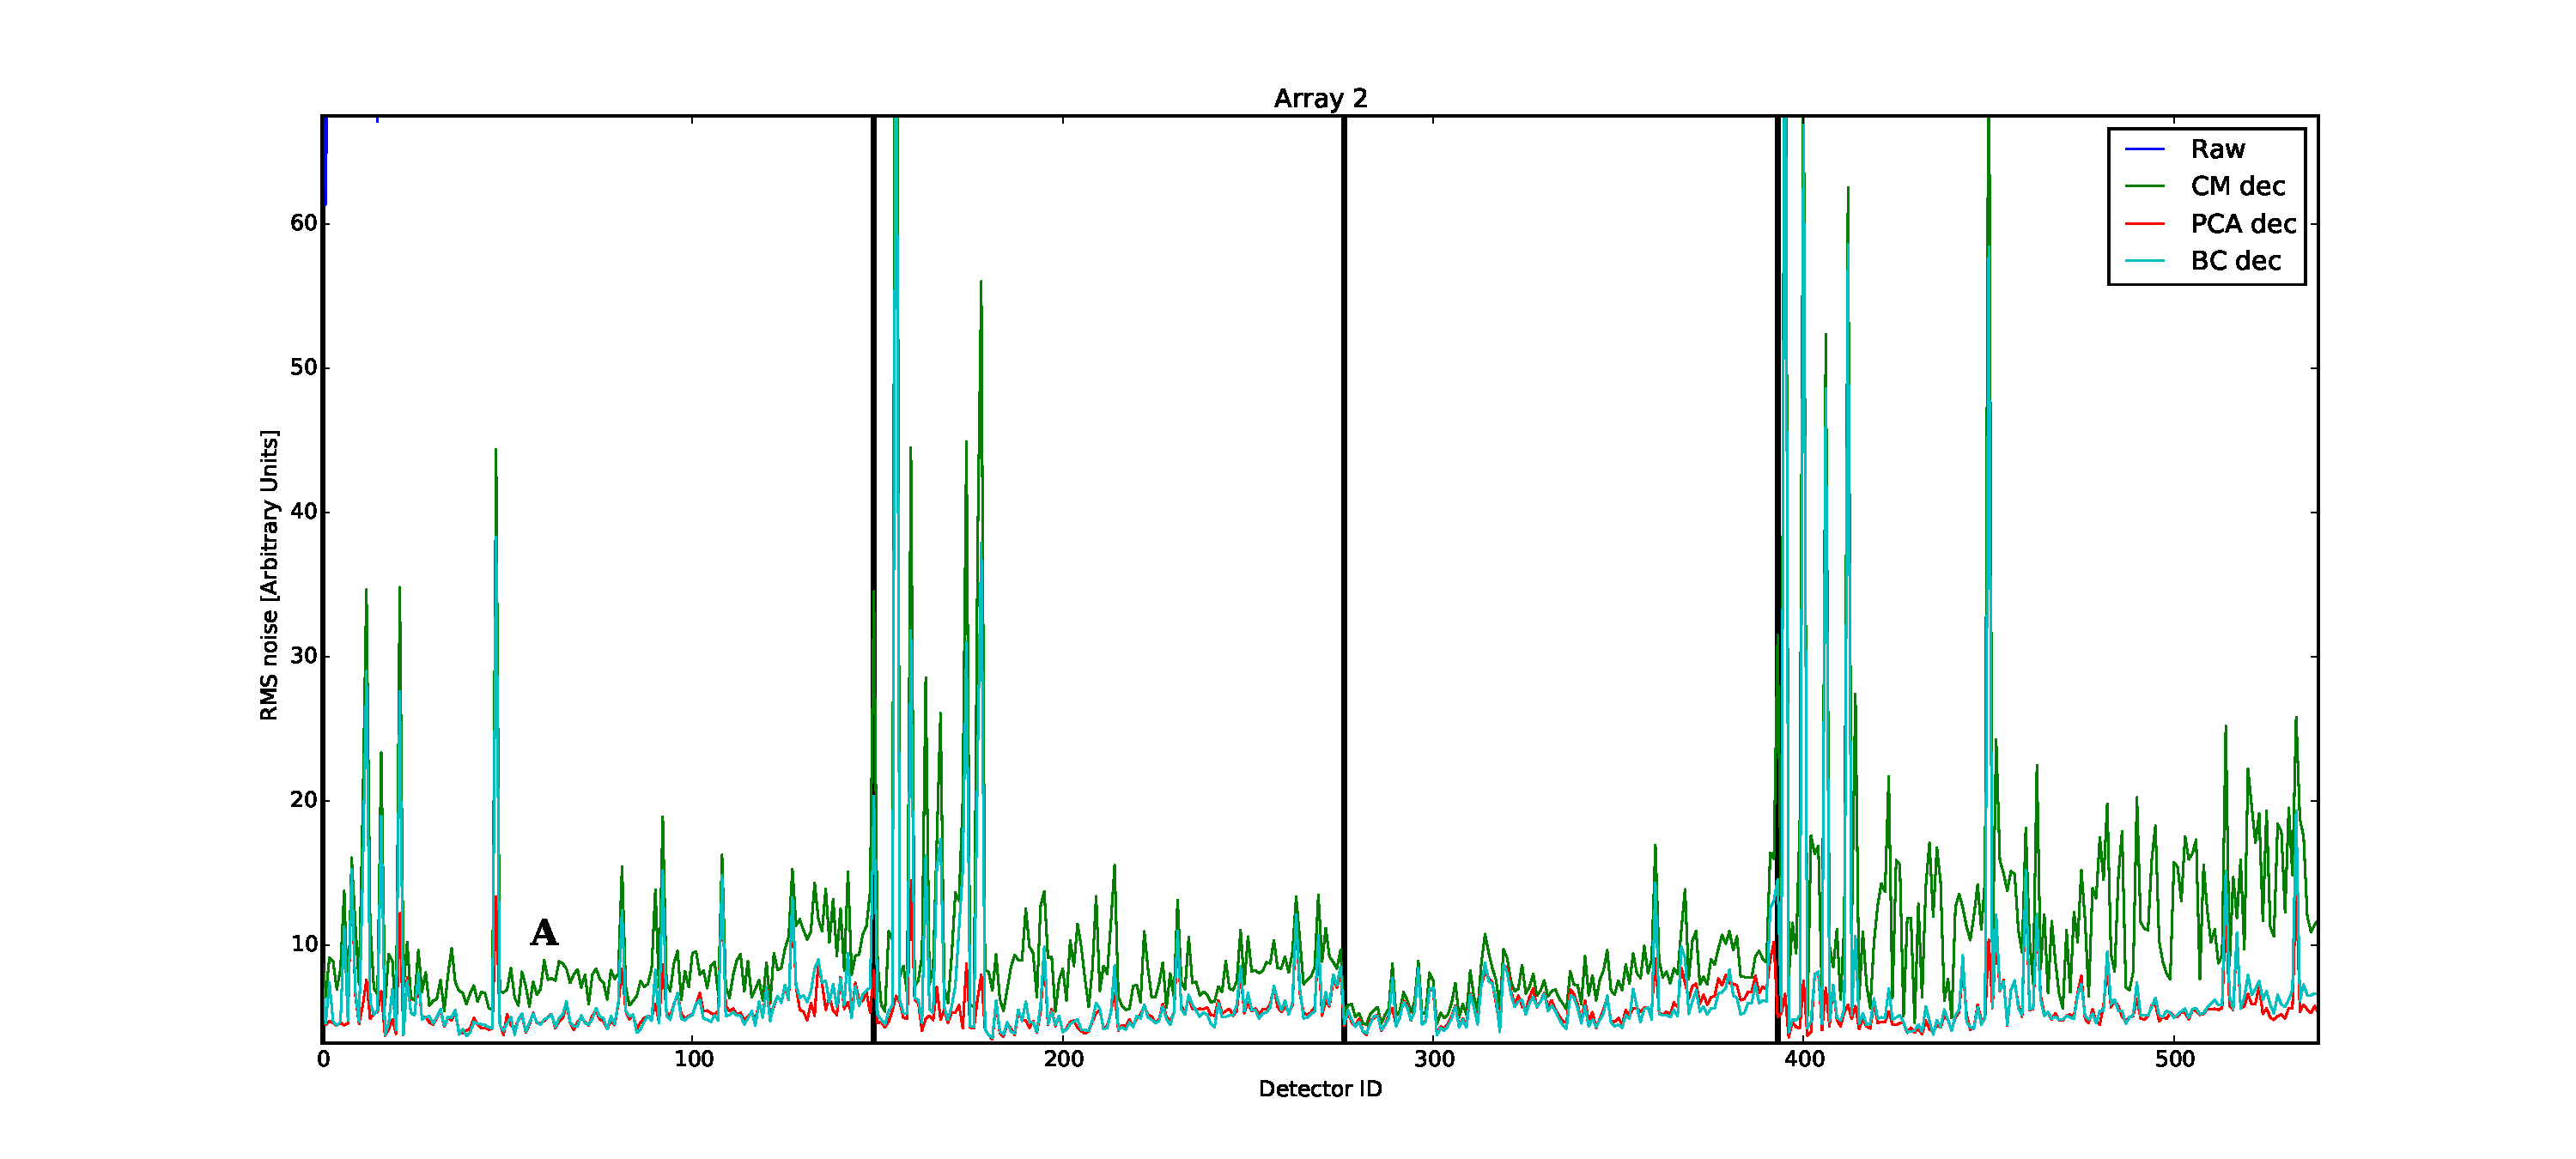
\includegraphics[width=0.3\textwidth]{Figures/NoiseTests/rms_TOI_array_2_20170228s151.pdf}
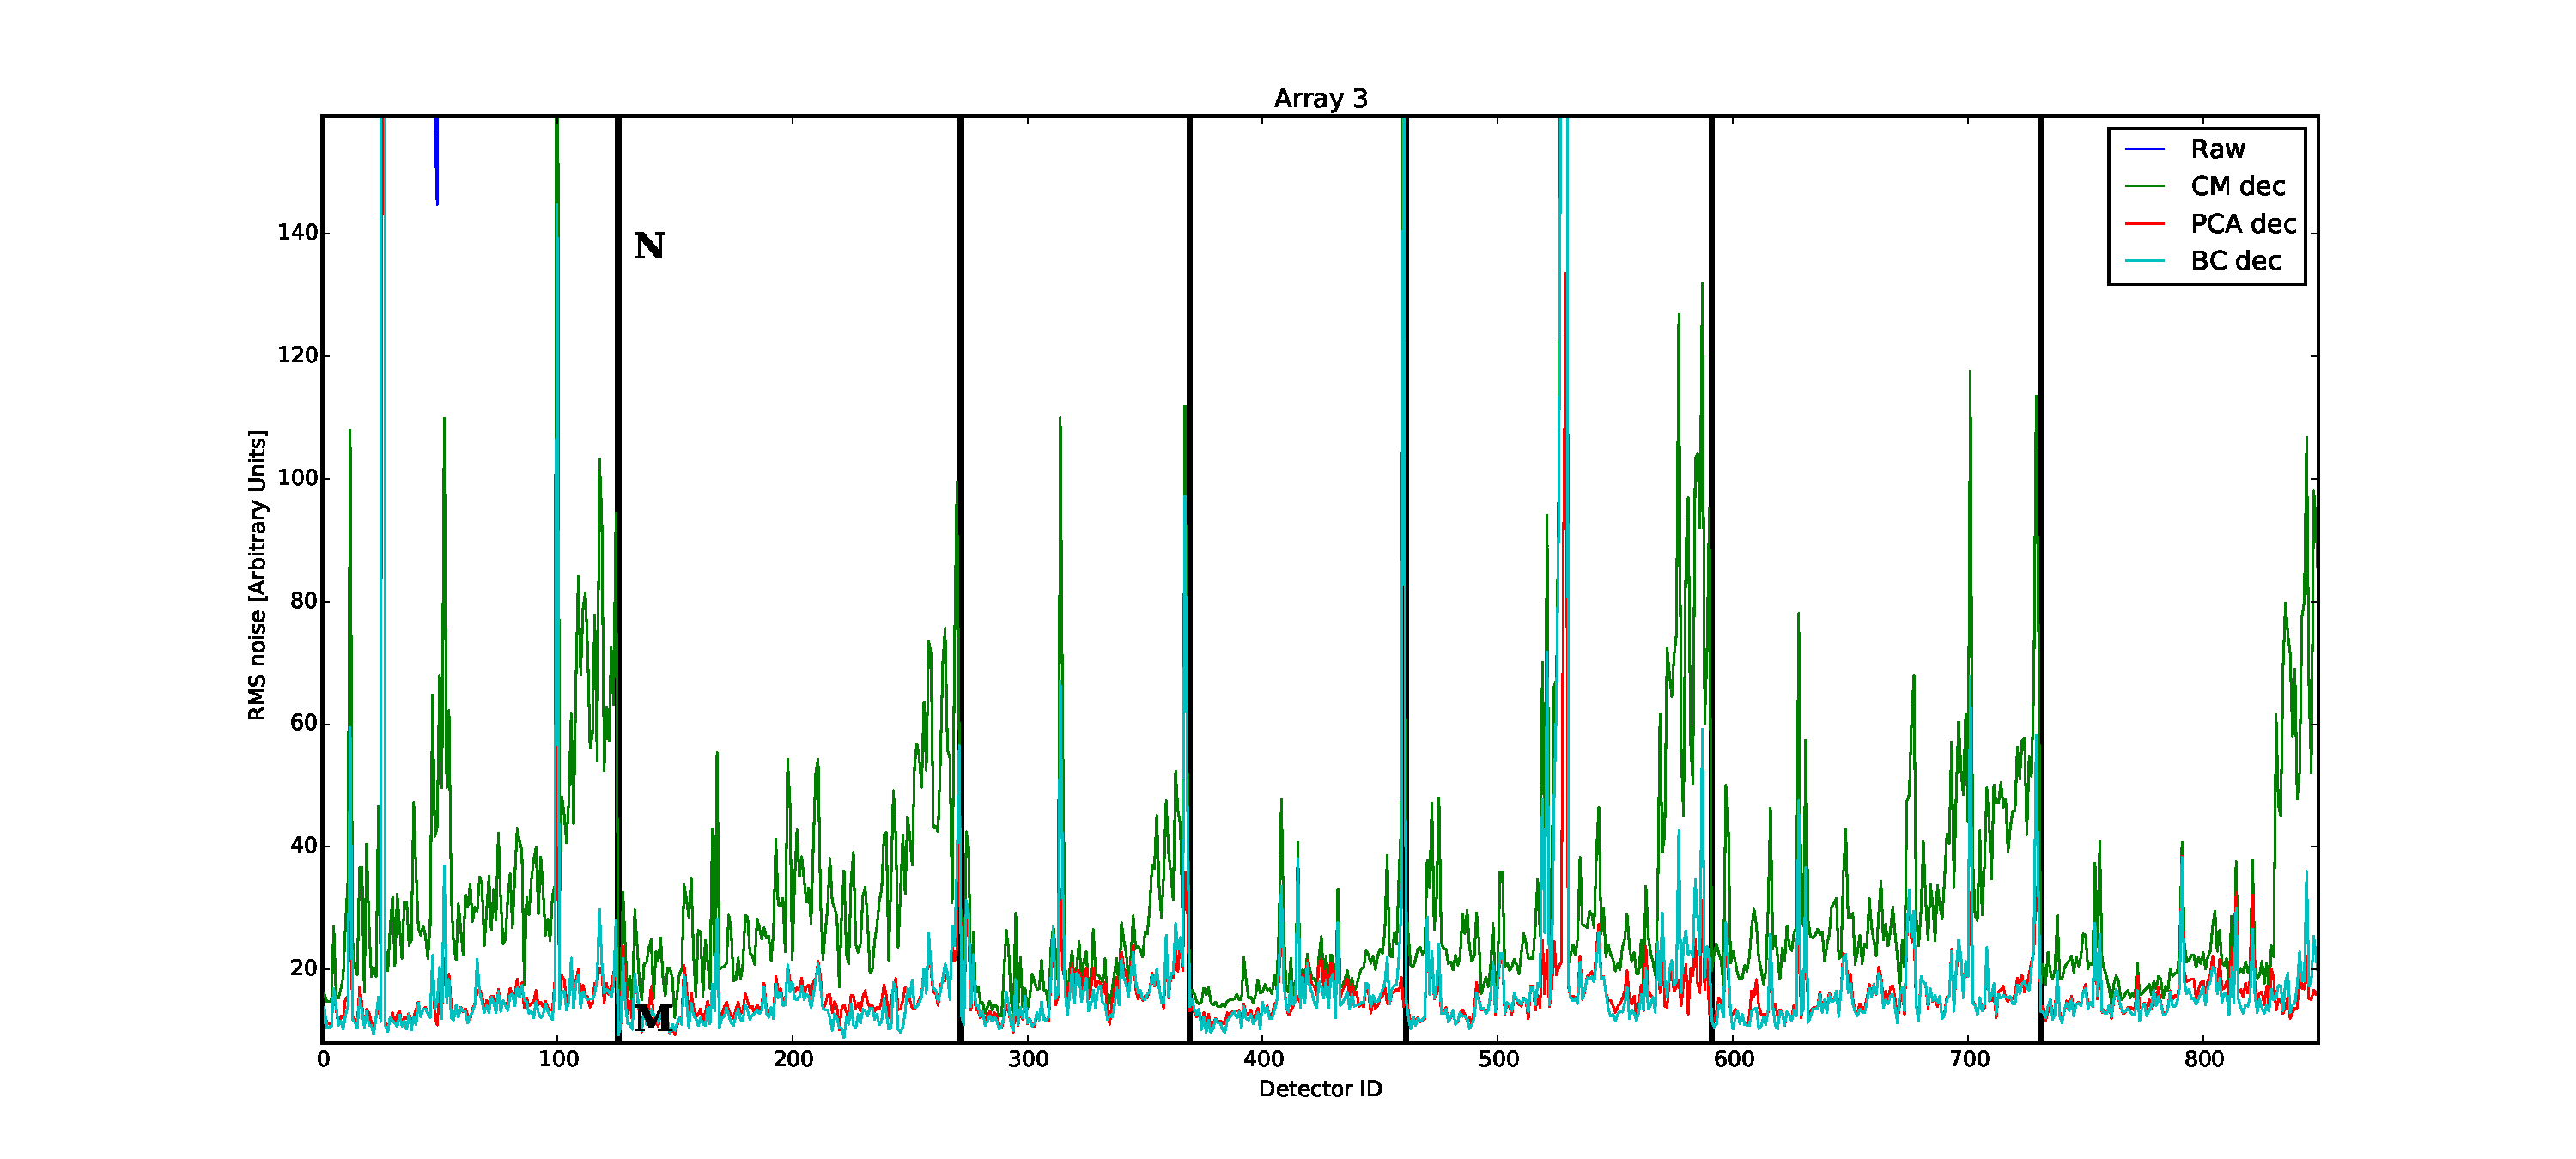
\includegraphics[width=0.3\textwidth]{Figures/NoiseTests/rms_TOI_array_3_20170228s151.pdf}
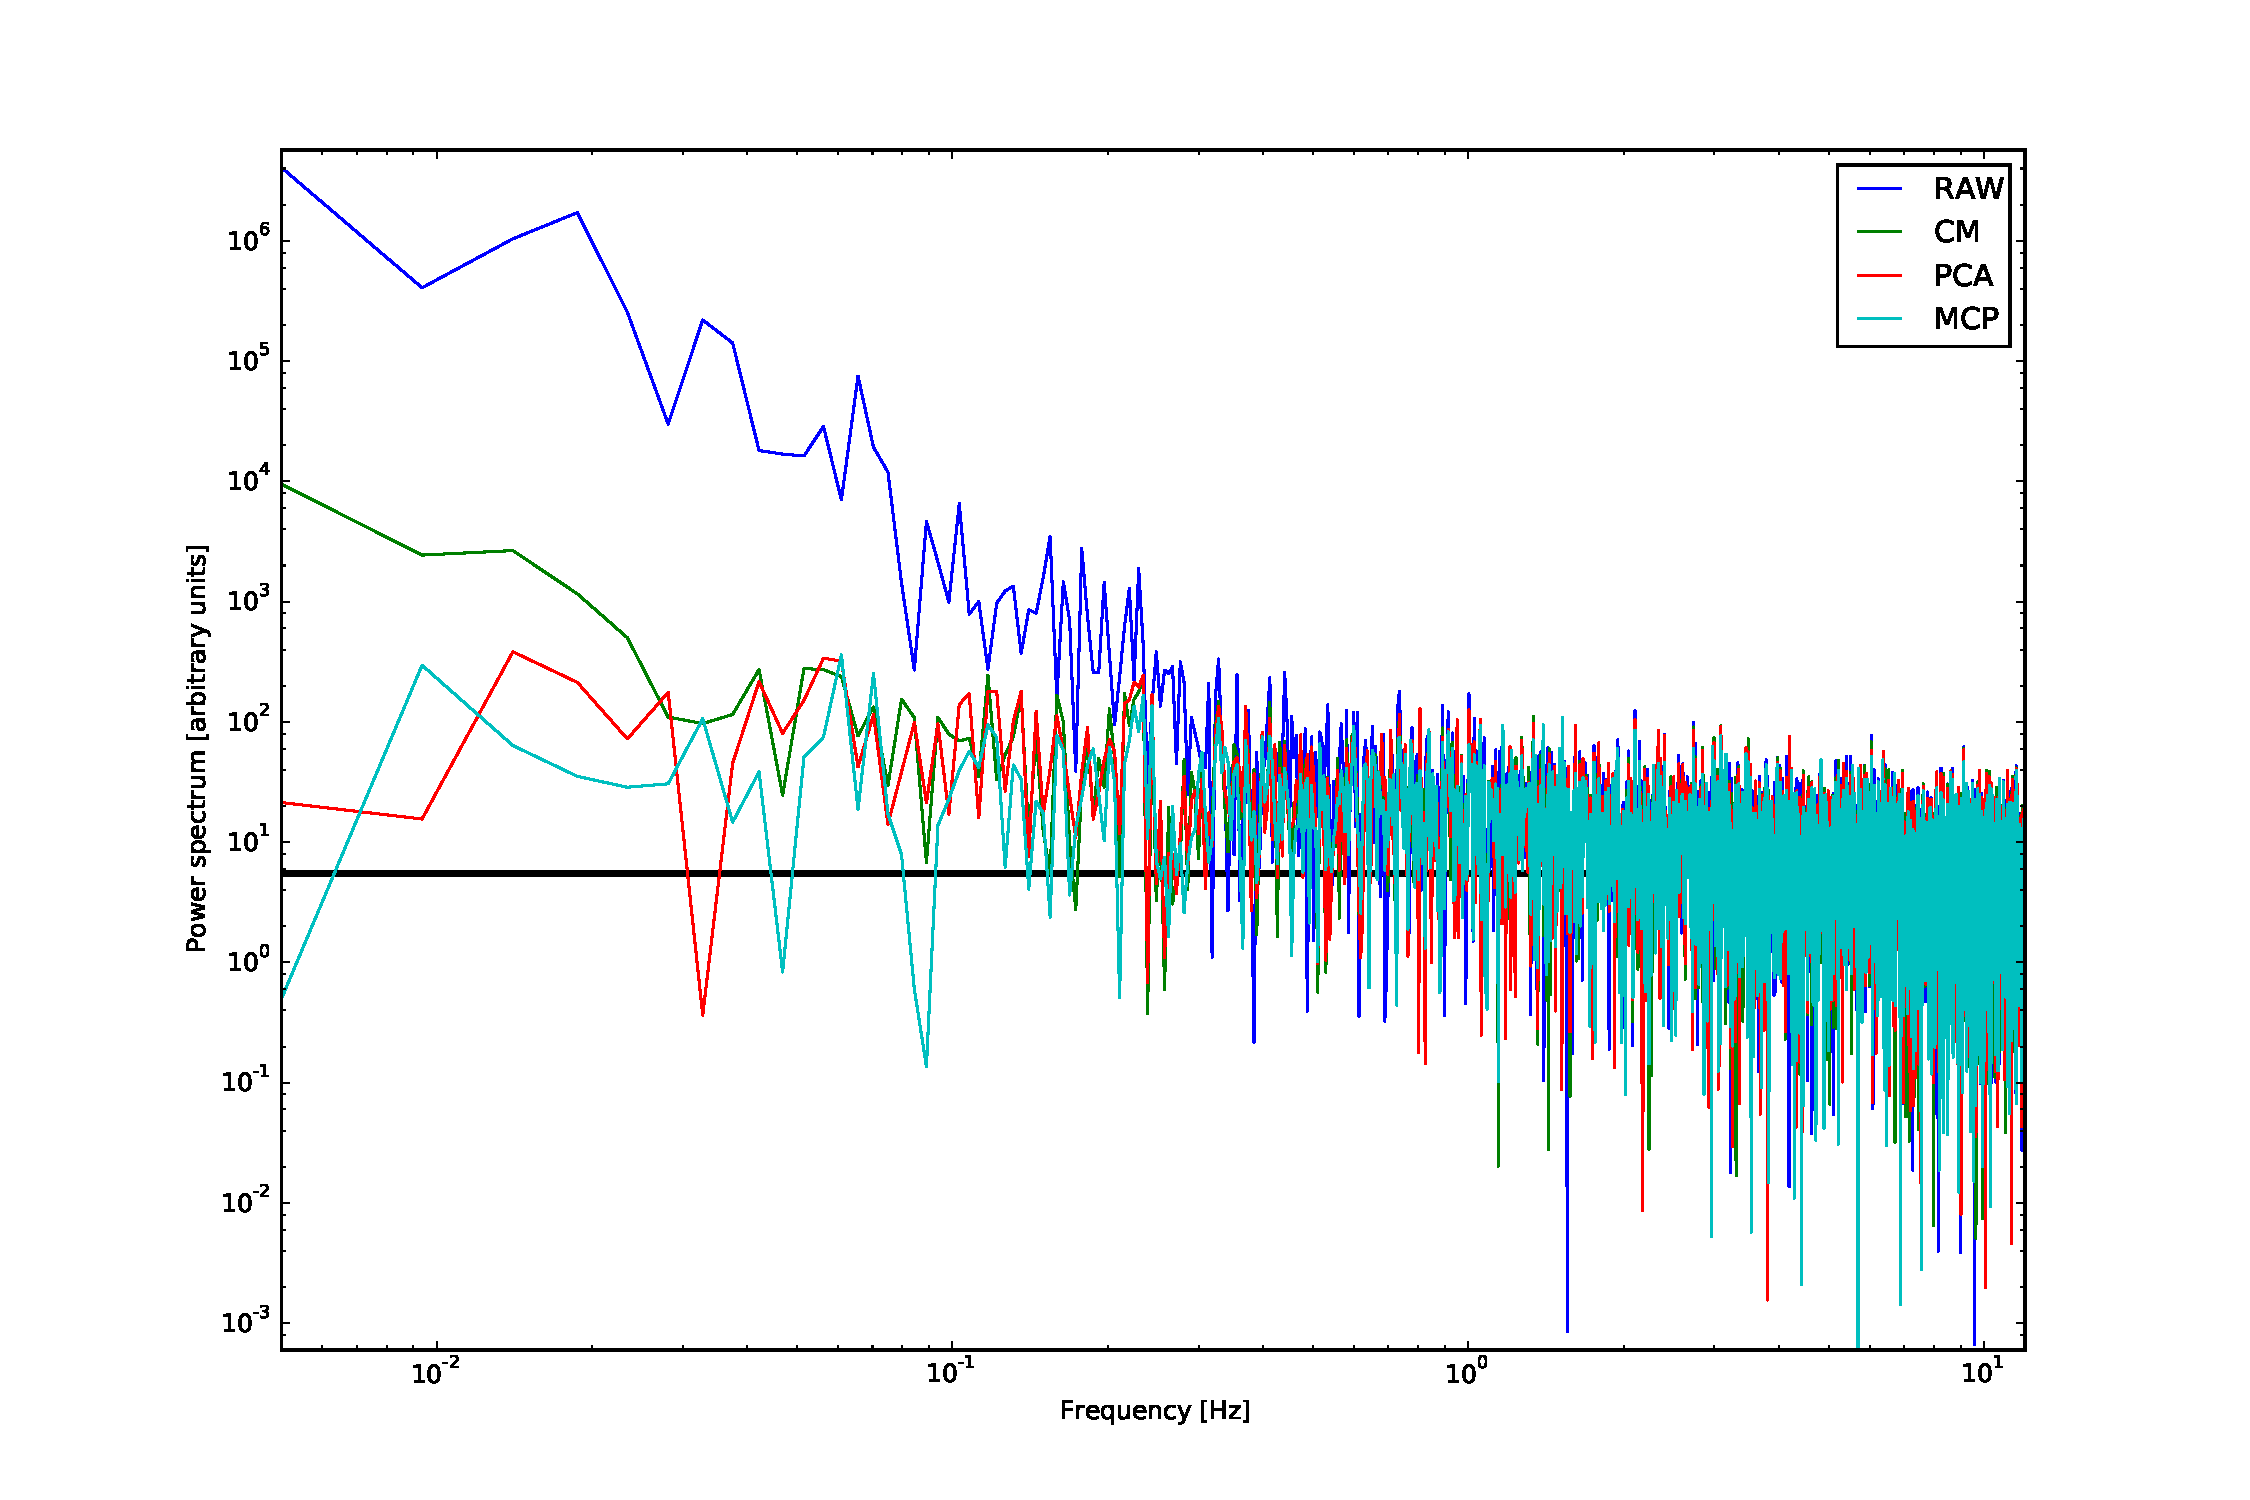
\includegraphics[width=0.3\textwidth]{Figures/NoiseTests/pws_TOI_array_1_20170228s151.pdf}
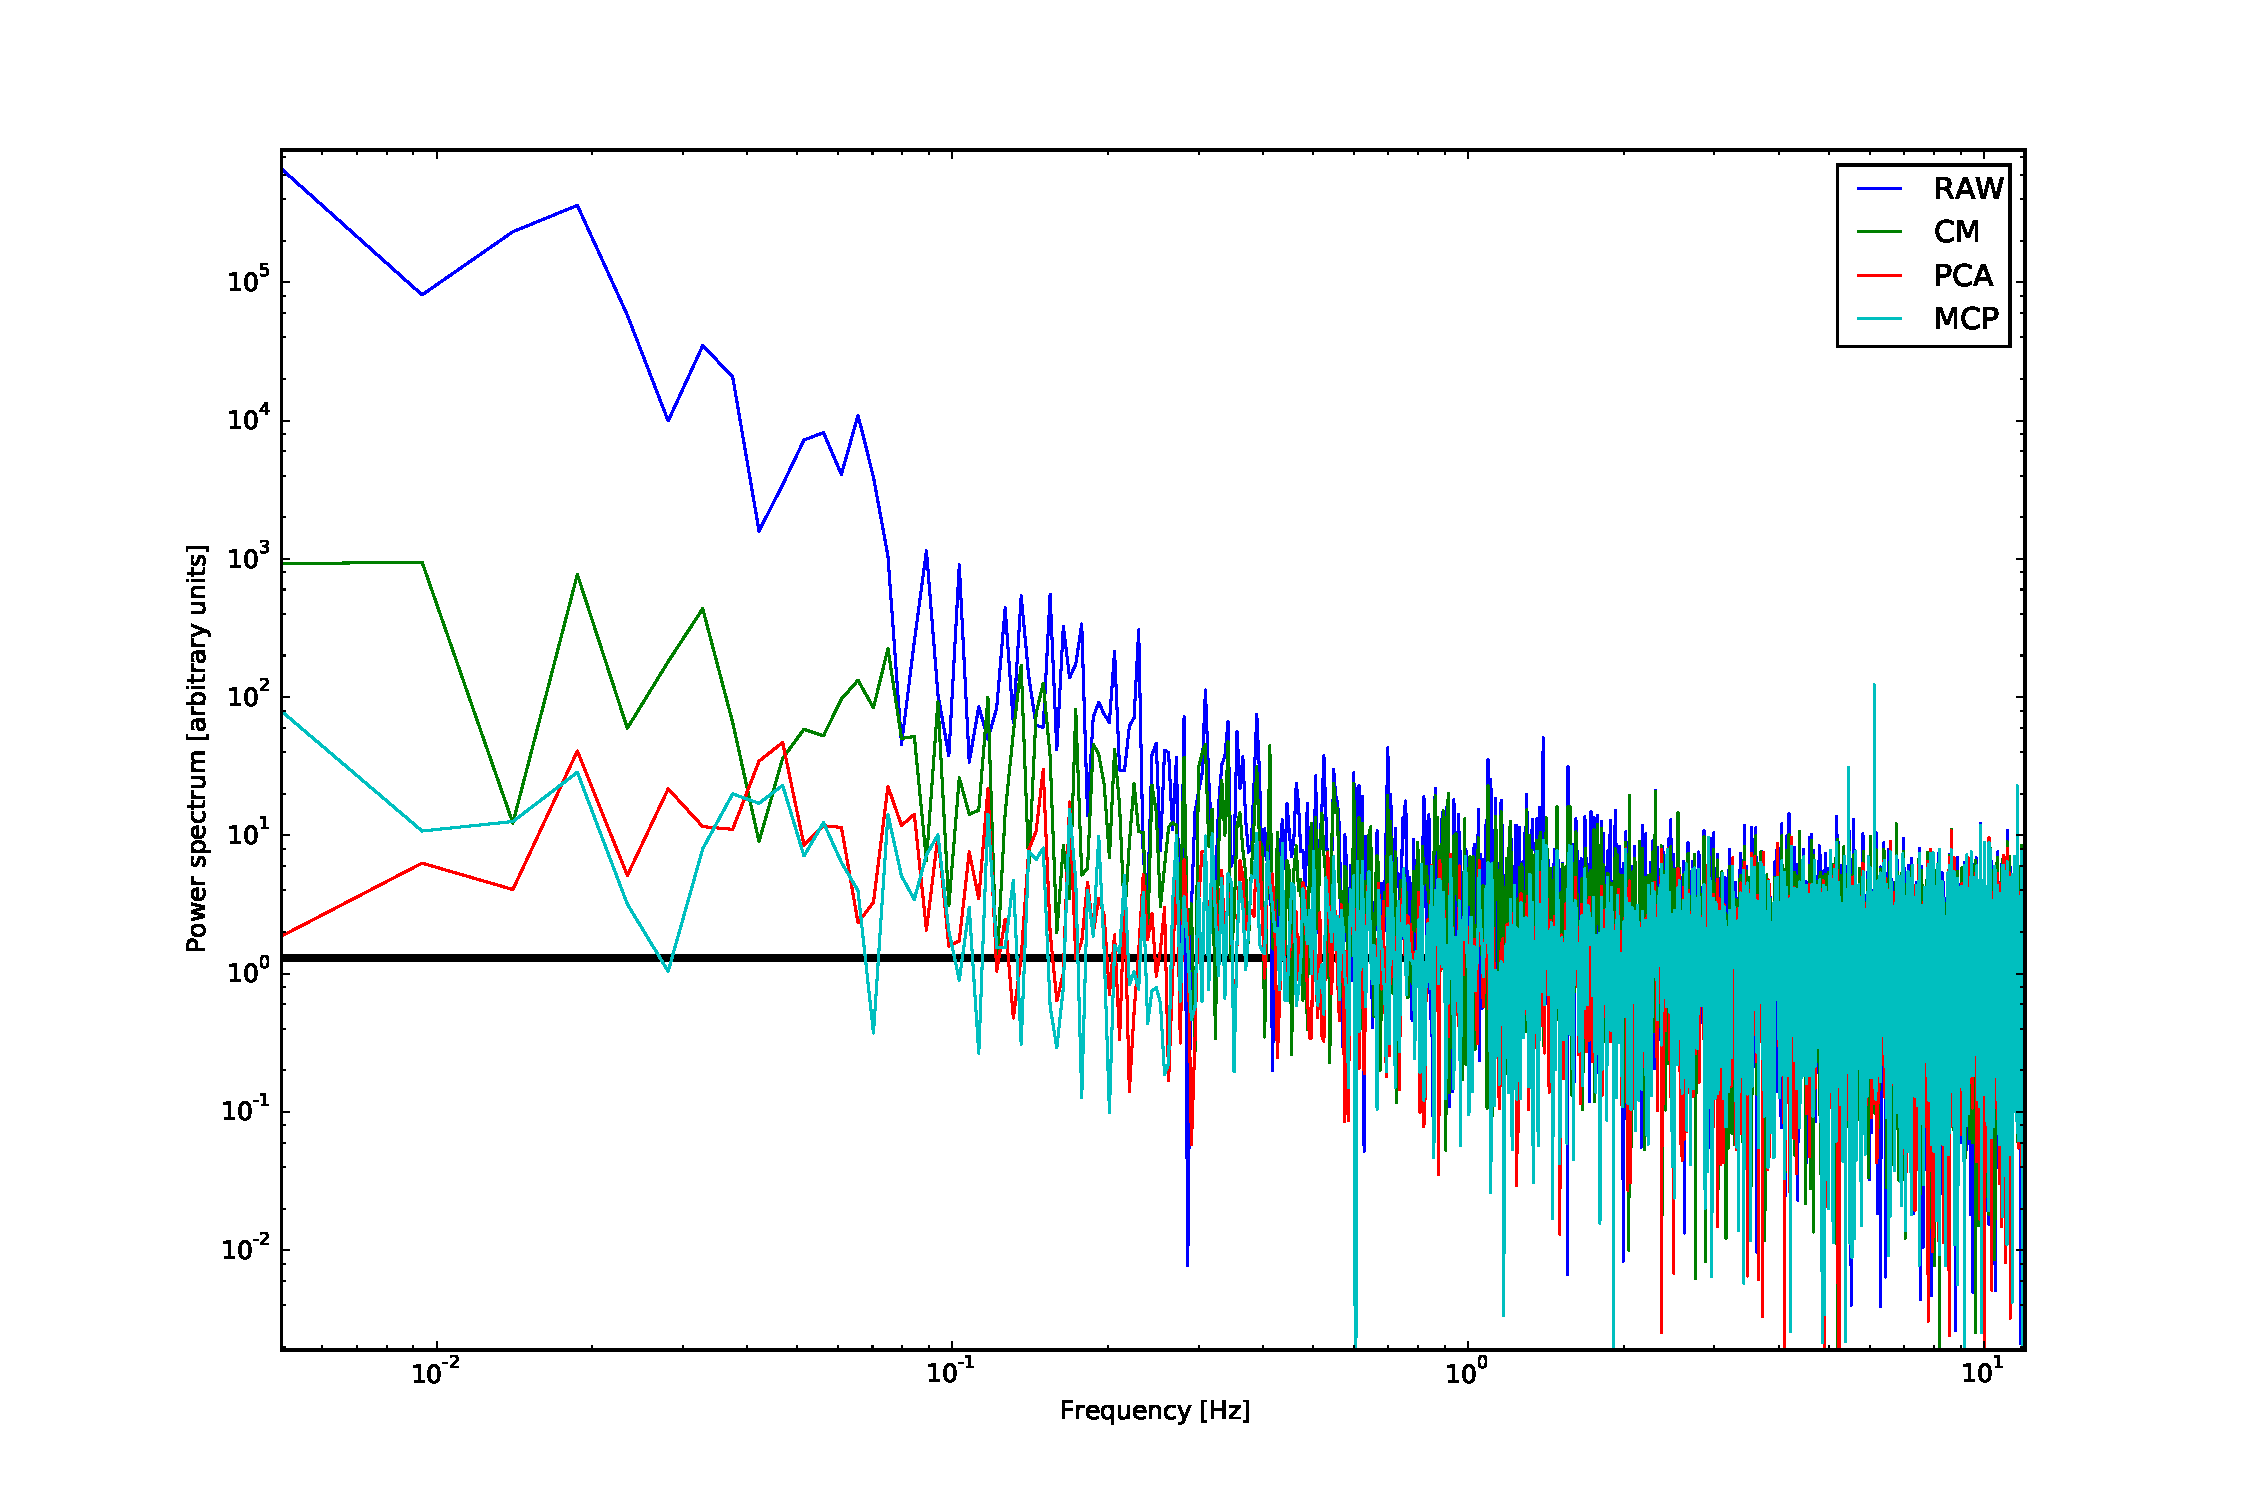
\includegraphics[width=0.3\textwidth]{Figures/NoiseTests/pws_TOI_array_2_20170228s151.pdf}
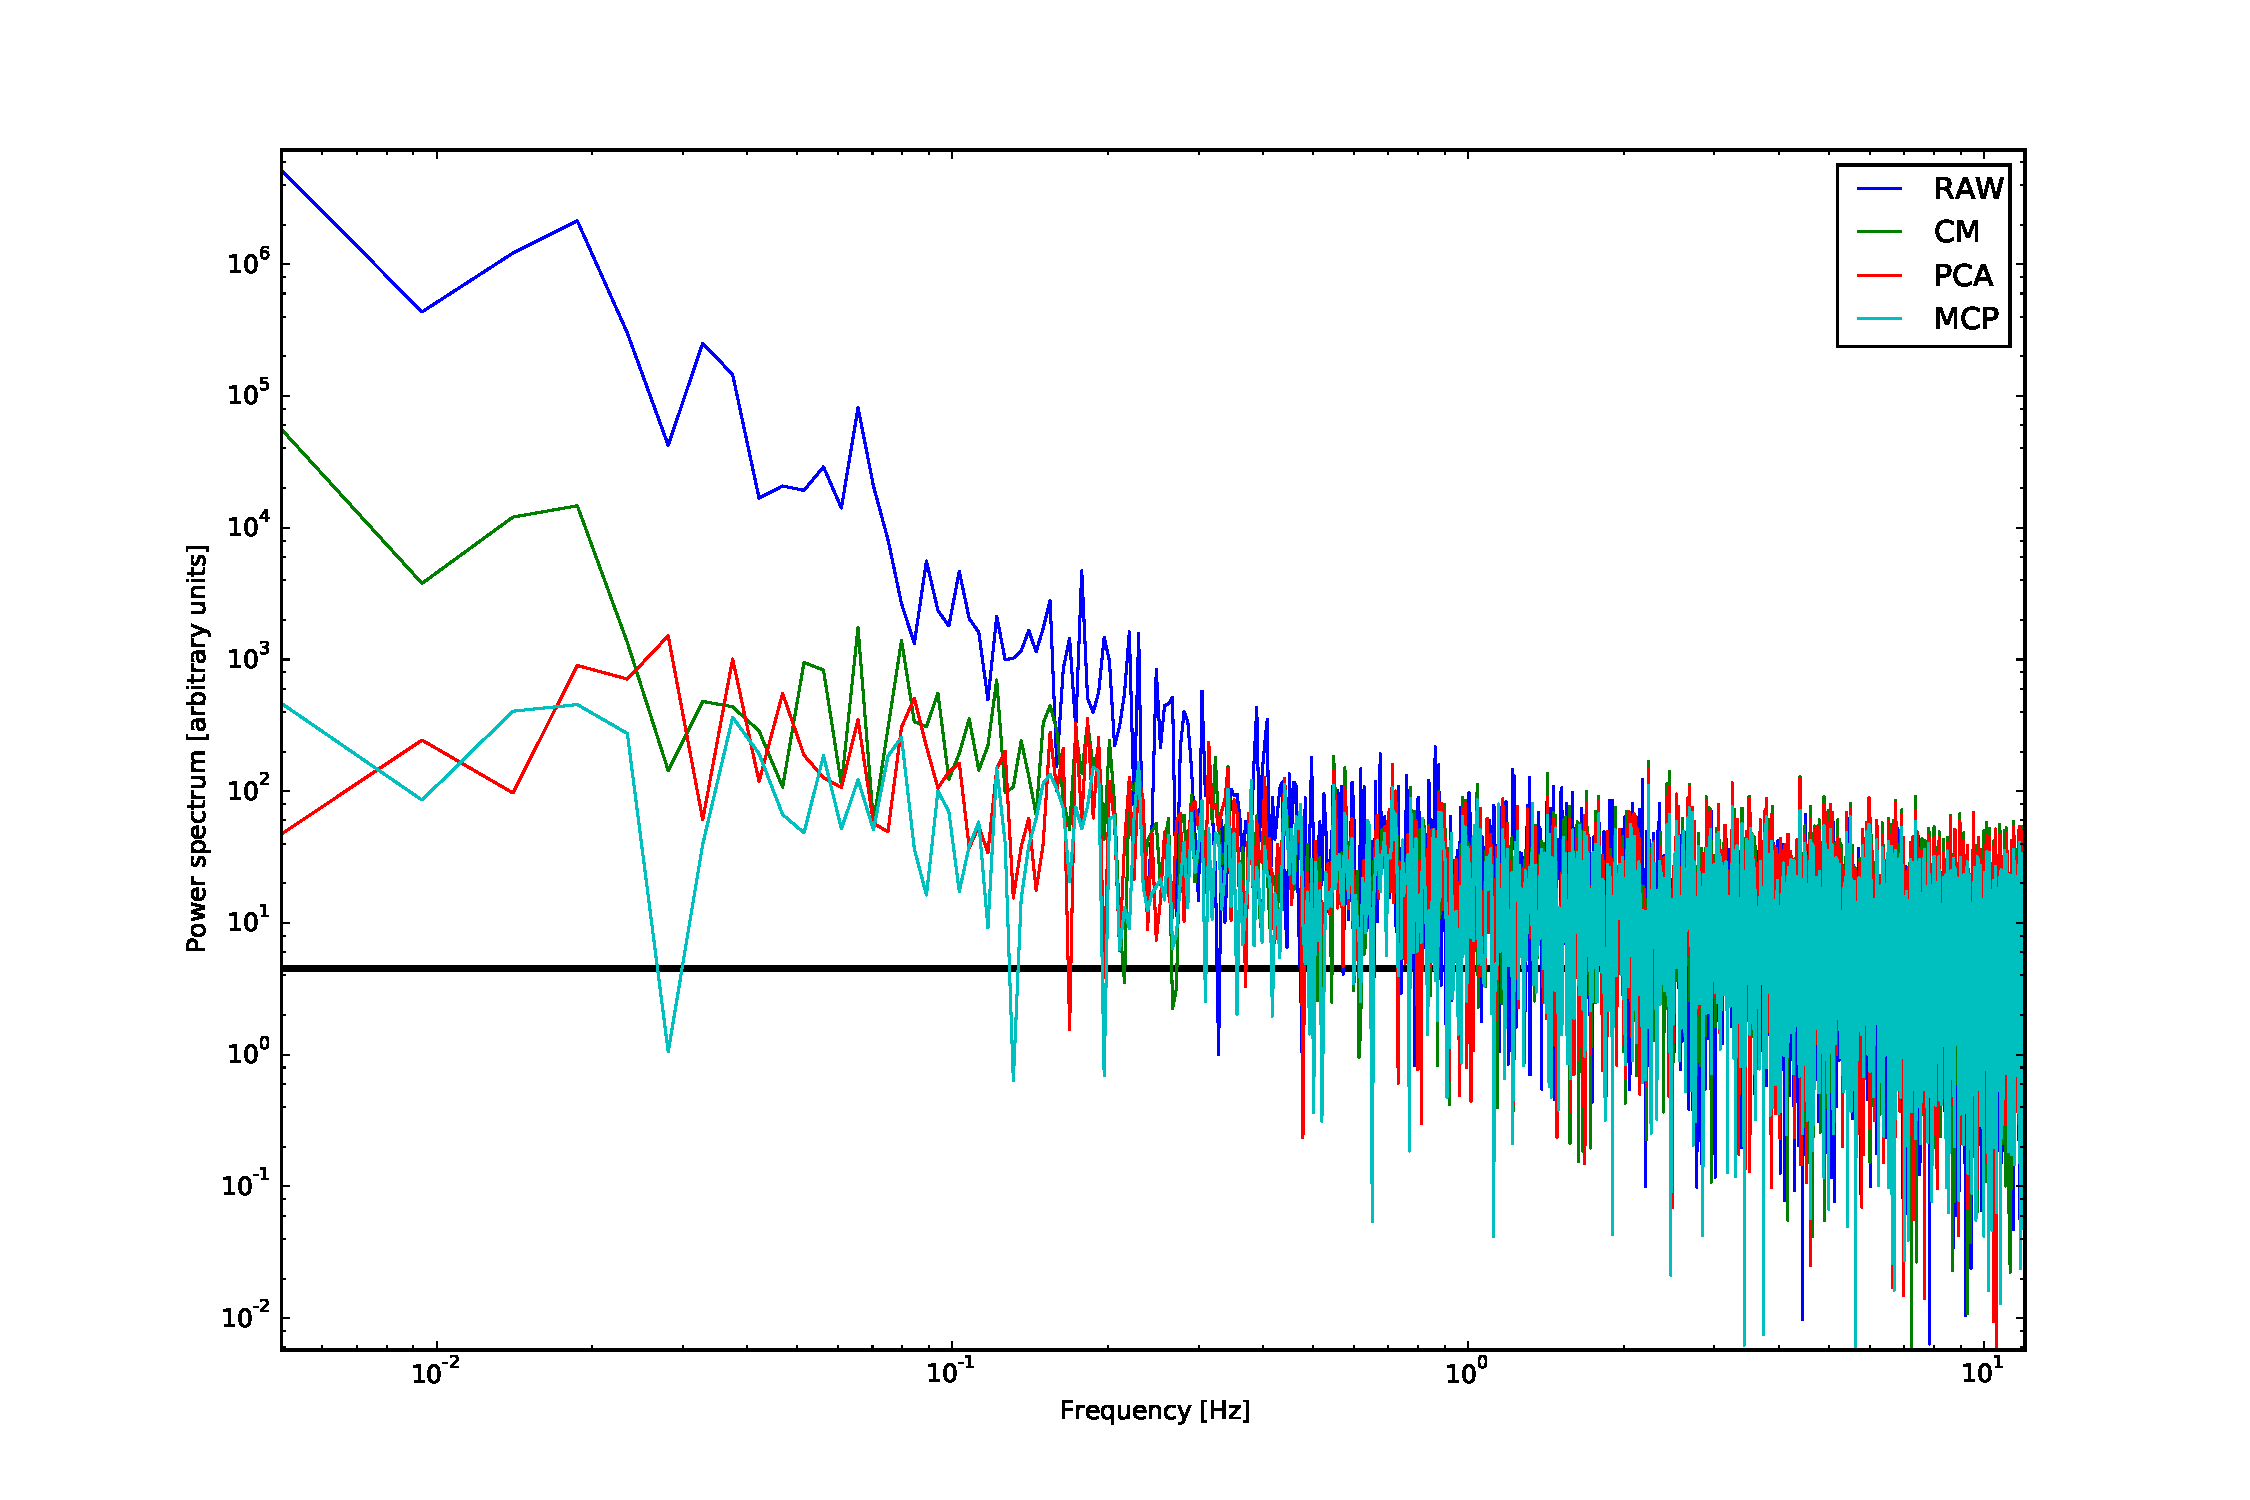
\includegraphics[width=0.3\textwidth]{Figures/NoiseTests/pws_TOI_array_3_20170228s151.pdf}

\end{center}
\caption[Noise RMS and power spectra]{From top to bottom and from left to right, we show the data rms and power spectra for the three NIKA2 arrays (A1, A2, and A3) for scan 20170228s150. The rms and power spectra are given for the raw data (blue), and for the CM (green), PCA (red) and BCP (cyan) decorrelated data. The vertical lines in the rms noise figures separate detectors from different readout electronic boxes. Whithin each electronic box the pixels are ordered with increasing resonant frequency across the electronic band. \label{rmspws}}
\end{figure}

In Figure \ref{rmspws} we present the rms noise and power spectra for the raw data, and the CMB, PCA and BCP decorrelated data. 
We observe that after decorralation we reduce significantly the rms of the noise. Equivalently, in $1/f$-like noise in the power spectra (principally due to atmospheric emission) is significantly reduced leading to nearly flat spectra down to 0.05 Hz, with larger $1/f$-like residual noise for the CM decorrelation method at lower frequencies. This is translated into a larger rms noise for this method with respect to the others. For the three arrays we find increasing noise with increasing resonant frequency withing each electronic box. This is probably related to the difference of gains between subbands in the readout electronics. We also find for the three arrays some noise bursts that are not fully consistent from one decorrelation method to another. \\

A more detailed study of the noise properties for improve the signal reconstruction is taking place taking profits of the qualitative findings described here. Report on this work will be made available to IRAM when the methodology is fully stablished.
